\section{Results}

The aim of this project has been to realize the double Fano cavity experimentally and investigate its transmission profile as a function of the incident wavelength. In this section I present the best results obtained and comment on these. Furthermore, I will outline challenges and obstacles that have been encountered, their implications on the data presented and my thoughts on immediate improvements for future experiments. 

The results obtained have been so through an iterative process realizing the theory presented in previous sections. For this reason, the structure of this section will outline this process and thus begin by an in depth spectral analysis of the Fano mirrors used, as a pair matching in optical parameters, and especially the guided-mode resonance wavelength, is crucial in order to realize the Fano resonance. When moving on to the results regarding cavity characterization I will begin by briefly verifying the results for the single Fano cavity presented by Mitra et al. in \cite{Mitra}. Finally, I will show experiemental results of the optical characterization of the double Fano cavity. 

\subsection{Fano mirror characterization}\label{sec:results_fano_mirror_characterization}

The first important step in realizing the double Fano cavity, is to locate a matching pair of Fano mirrors. A substantial spectral overlap is necessary to excite a Fano resonance including both guided-modes, as explained in section \ref{sec:spectral_detuning}. For this reason the Fano mirrors considered were all fabricated externally by \emph{Norcada} and from the same "batch", as these were initially considered to have a greater probability of having similar physical attributes. Many Fano mirrors were thus characterized during the process of finding a match, and the pair eventually chosen to move forward with were denoted \emph{G1} and \emph{G2}. 

\begin{figure}[h!]
    \centering
    \begin{subfigure}[b]{0.49\textwidth}
        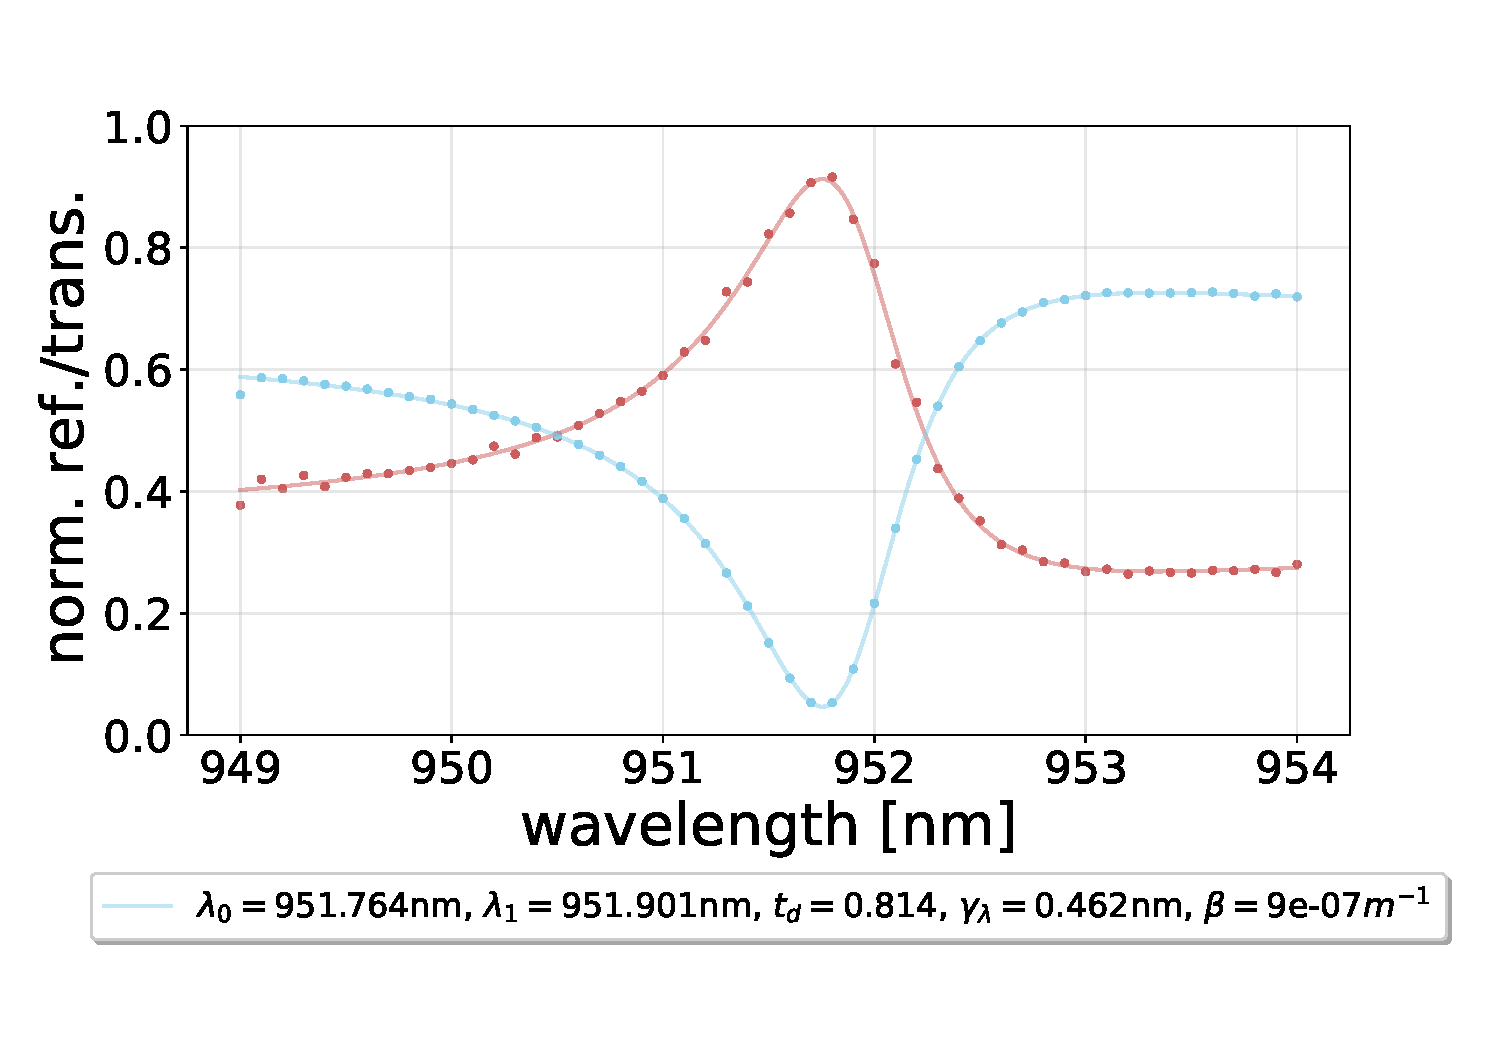
\includegraphics[width=\textwidth]{figures/results/M3:M5/M5:G1_initial_spectrum.pdf}
        \caption{}
        \label{}
    \end{subfigure}
    \begin{subfigure}[b]{0.49\textwidth}
        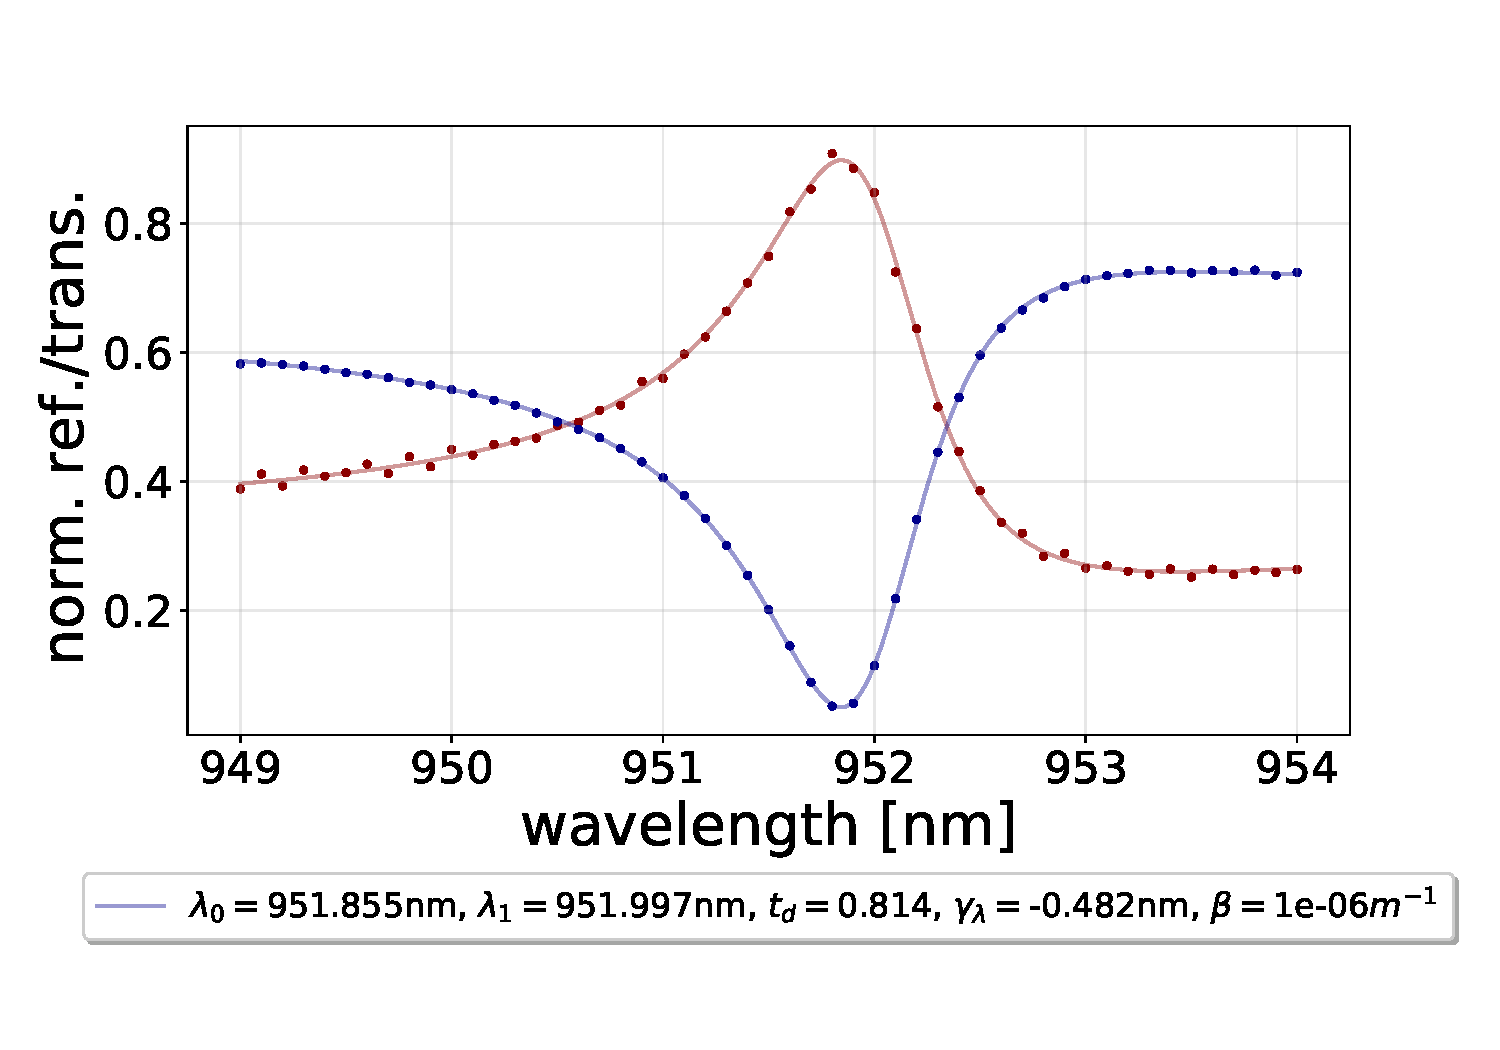
\includegraphics[width=\textwidth]{figures/results/M3:M5/M3:G2_initial_spectrum.pdf}
        \caption{}
        \label{}
    \end{subfigure}
    \caption{(a) shows the normalized reflection and transmission spectra of Fano mirror G1 along with its optical parameters found as fitting parameters from a least squares fit to the model derived in section \ref{sec:fano_mirror}. (b) shows the same for Fano mirror G2. Spectra of Fano mirrors that were characterized but not included in further experiments can be found in Appendix \ref{appendix:Additional Fano mirror characterizations}.}
    \label{fig:individual_G1_and_G2_spectra}
\end{figure}

Figure \ref{fig:individual_G1_and_G2_spectra} shows the individual measured normalized reflection and transmission spectra of G1 and G2 together with a least squares fit to the model derived in section \ref{sec:fano_mirror}. The corresponding optical parameters for each Fano mirror were found as the following.

\newpage
Fitting parameters for G1:
\begin{equation}
    \begin{split}
        \lambda_{0,G1} &= 951.764 \text{nm}, \:\: \lambda_{1,G1} = 951.901 \text{nm},\:\: t_d = 0.814, \\&r_d = 0.575, \:\:  \gamma_{\lambda} = 0.462 \text{nm},\:\: \beta = 9 \cdot 10^{-7} \text{nm}^{-1}.
    \end{split}
    \label{eq:G1_params}
\end{equation}

Fitting parameters for G2:
\begin{equation}
    \begin{split}
        \lambda_{0,G2} &= 951.855 \text{nm}, \:\: \lambda_{1,G2} = 951.997 \text{nm},\:\: t_d = 0.814, \\&r_d = 0.570, \:\:  \gamma_{\lambda} = 0.482 \text{nm},\:\: \beta = 1 \cdot 10^{-6} \text{nm}^{-1}.
    \end{split}
    \label{eq:G2_params}
\end{equation}

To evaluate and compare the parameters to determine whether the two Fano mirrors are in fact a good match, they are both shown alongside eachother in figure \ref{fig:G1_and_G2_spectral_comparison} for spectral comparison. Each their resonance wavelengths $\lambda_0$ are indicated on the figure and the detuning can thus be estimated as 
\begin{equation}
    \Delta = \left|\lambda_{0,G2} - \lambda_{0,G1}\right| = 951.855 \text{nm} - 951.764 \text{nm} = 0.091 \text{nm}.
    \label{eq:G1/G2_detuning}
\end{equation}

Here we remember that the additional fitting parameters, namely $t_d$, $r_d$, $\gamma_{\lambda}$ and $\beta$, are assumed identical in the model for the double Fano cavity outlined in section \ref{sec:double_fano_lw_theory} and these are thus compared in a more qualitative manner. Whether the parameters in eqs. (\ref{eq:G1_params}) and (\ref{eq:G2_params}) can be assumed identical is completely individual to the given experiment and the corresponding acceptable margins. In order to move forward, G1 and G2 are assumed to only differ in guided-mode resonance wavelength.

\begin{figure}[h!]
    \centering
    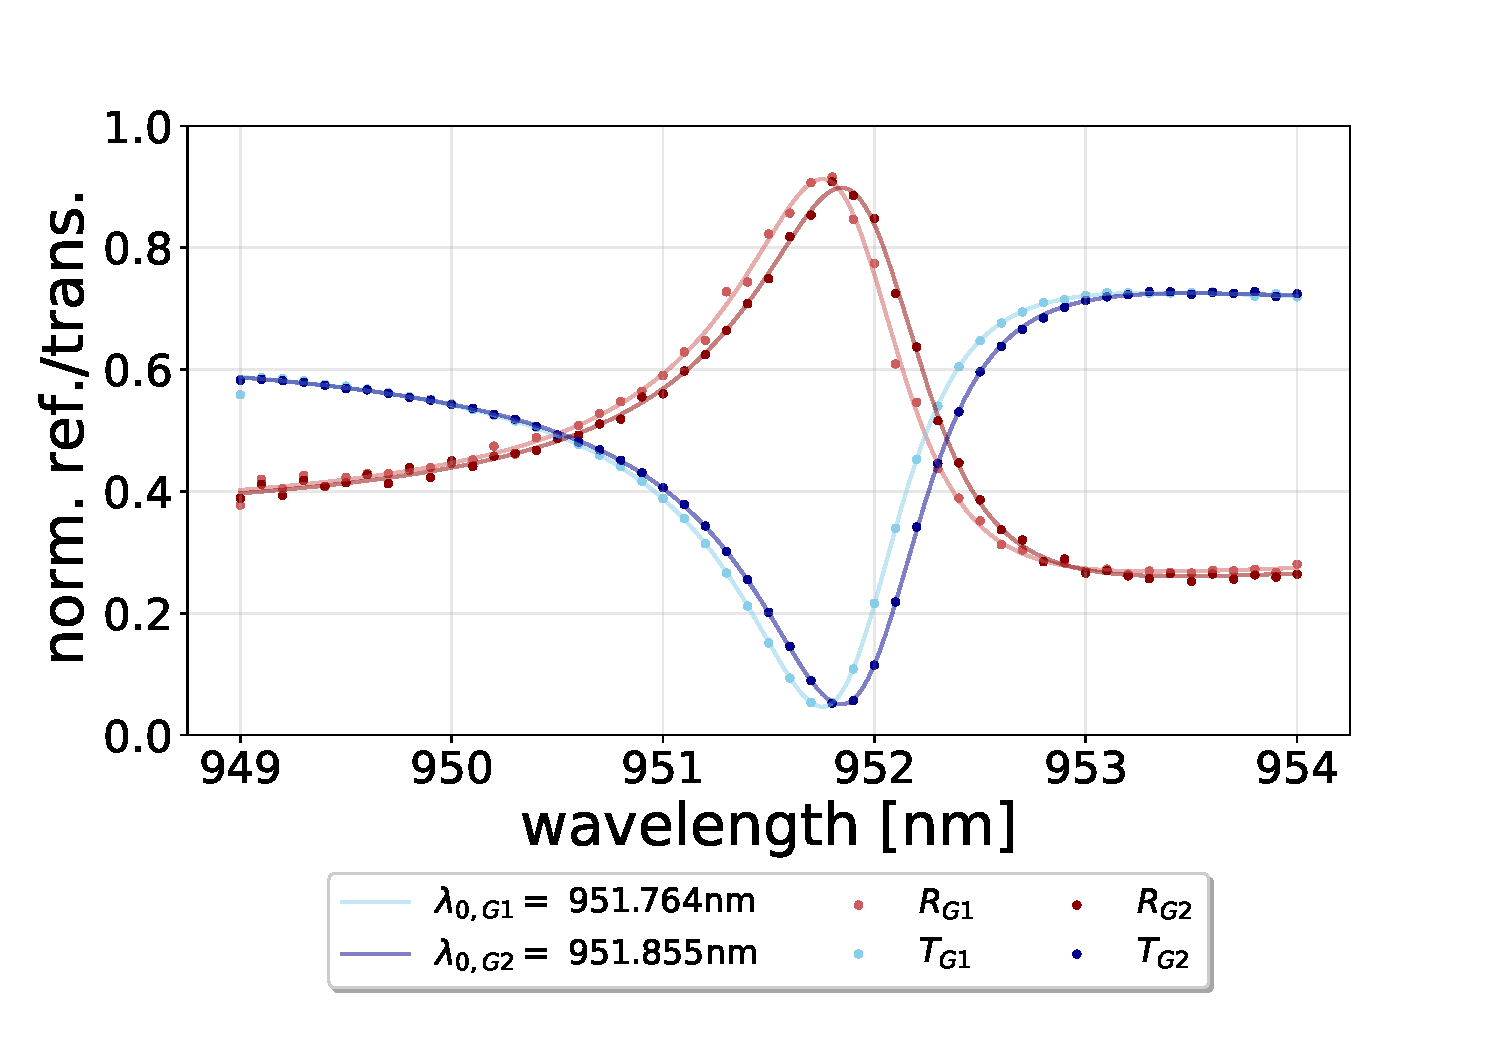
\includegraphics[width=0.7\textwidth]{figures/results/M3:M5/M3:M5_initial_spectra.pdf}
    \caption{Spectral comparison of Fano mirrors G1 and G2. The spectra are the same shown in figure \ref{fig:individual_G1_and_G2_spectra}.}
    \label{fig:G1_and_G2_spectral_comparison}
\end{figure}

As is shown in section \ref{sec:spacial_detuning}, a spectral detuning leads to a spatial detuning, meaning that the cavity length corresponding to the guided-mode resonance wavelength for G1 and G2 are not identical as they have a non-zero detuning $\Delta$. To sustain a Fano resonance it is equally important, and in fact equivalent to the spectral overlap, that the Fano mirrors have overlapping cavity transmission profiles as a function of the cavity length. Figure \ref{fig:G1/G2_length_scan} shows the simulated double Fano transmission of a cavity consisting of G1 and G2 for lengths corresponding to their guided-mode resonance wavelengths. It is readily seen that the two transmission profiles overlap for the included example of a cavity of length $l \approx 30 \mu m$.

\begin{figure}[h!]
    \centering
    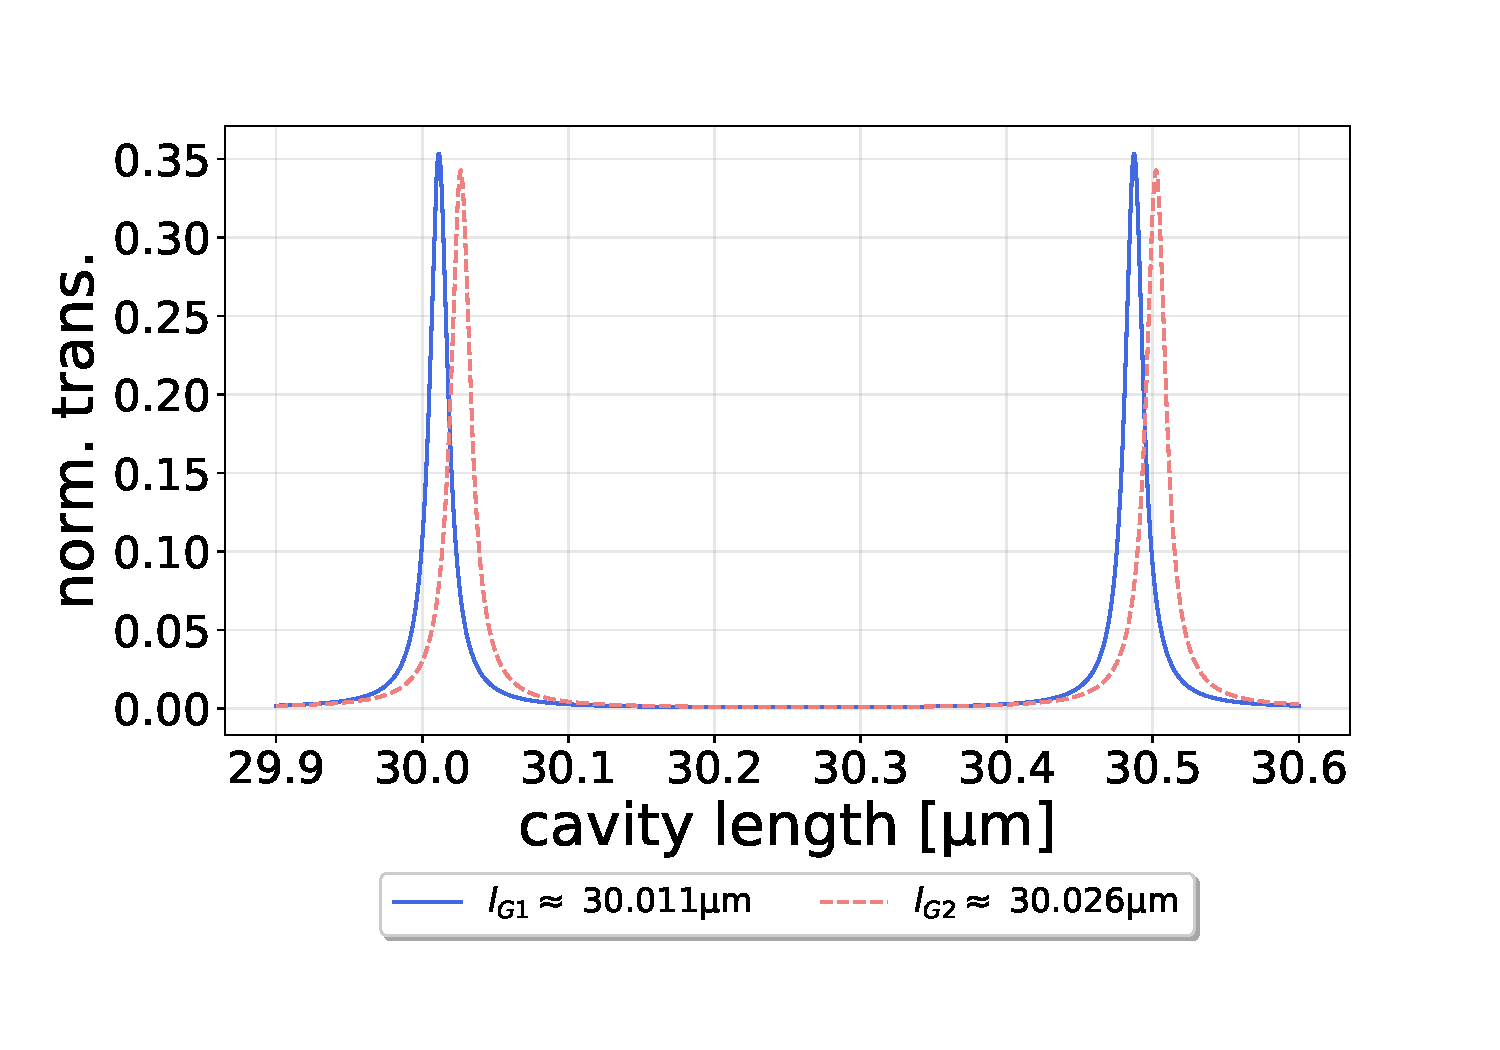
\includegraphics[width=0.7\textwidth]{figures/results/M3:M5_length_scan_sim_30um.pdf}
    \caption{Simulated length scans of double Fano cavities with incident wavelengths of $\lambda_{0,G1}$ and $\lambda_{0,G2}$. The cooresponding lengths determined from the scans are denoted $l_{G1}$ and $l_{G2}$, respectively.}
    \label{fig:G1/G2_length_scan}
\end{figure}

\clearpage
\subsection{The single Fano cavity}\label{sec:the_single_fano_cavity_results}

We recall that the single fano cavity consists of a Fano mirror and a broadband mirror in a plane-plane configurations where each mirror is perpendicular to the optical axis. The single Fano cavity configuration is briefly outlined in section \ref{sec:cavity_measurements} and otherwise shown in \cite{Mitra}, it however resembles the double Fano cavity setup shown in figure \ref{fig:cavity_setup}, except only the bottom two xy-stages are used, and the top ones are therefore removed.   

The mirror used is a high relfective (HR) broadband mirror with a reflectivity of $99.7\%$, meaning that effectively all intrinsic cavity losses can be assumed to be associated with the Fano mirror. The Fano mirror used is G1 characterized in section \ref{sec:results_fano_mirror_characterization}. 

Figure \ref{fig:single_fano_fsr_scans} shows examples of off-resonance spectra of the single Fano cavity, with corresponding fits to the Fabry-Perot transmission function, in order to determine the cavity length from the measured FSR. Figure \ref{fig:short_single_fano_FSR} shows the off-resonance spectrum for a cavity of length $l = 57.40 \pm 1.55 \mu m$, while figure \ref{fig:long_single_fano_FSR} shows the same for a cavity length of $l = 211.98 \pm 3.16 \mu m$. The errors are determined as the errors of the fit, found as the squareroot of the diagonal of the corresponding covariance matrices.

\begin{figure}[h!]
    \centering
    \begin{subfigure}[b]{0.49\textwidth}
        \centering
        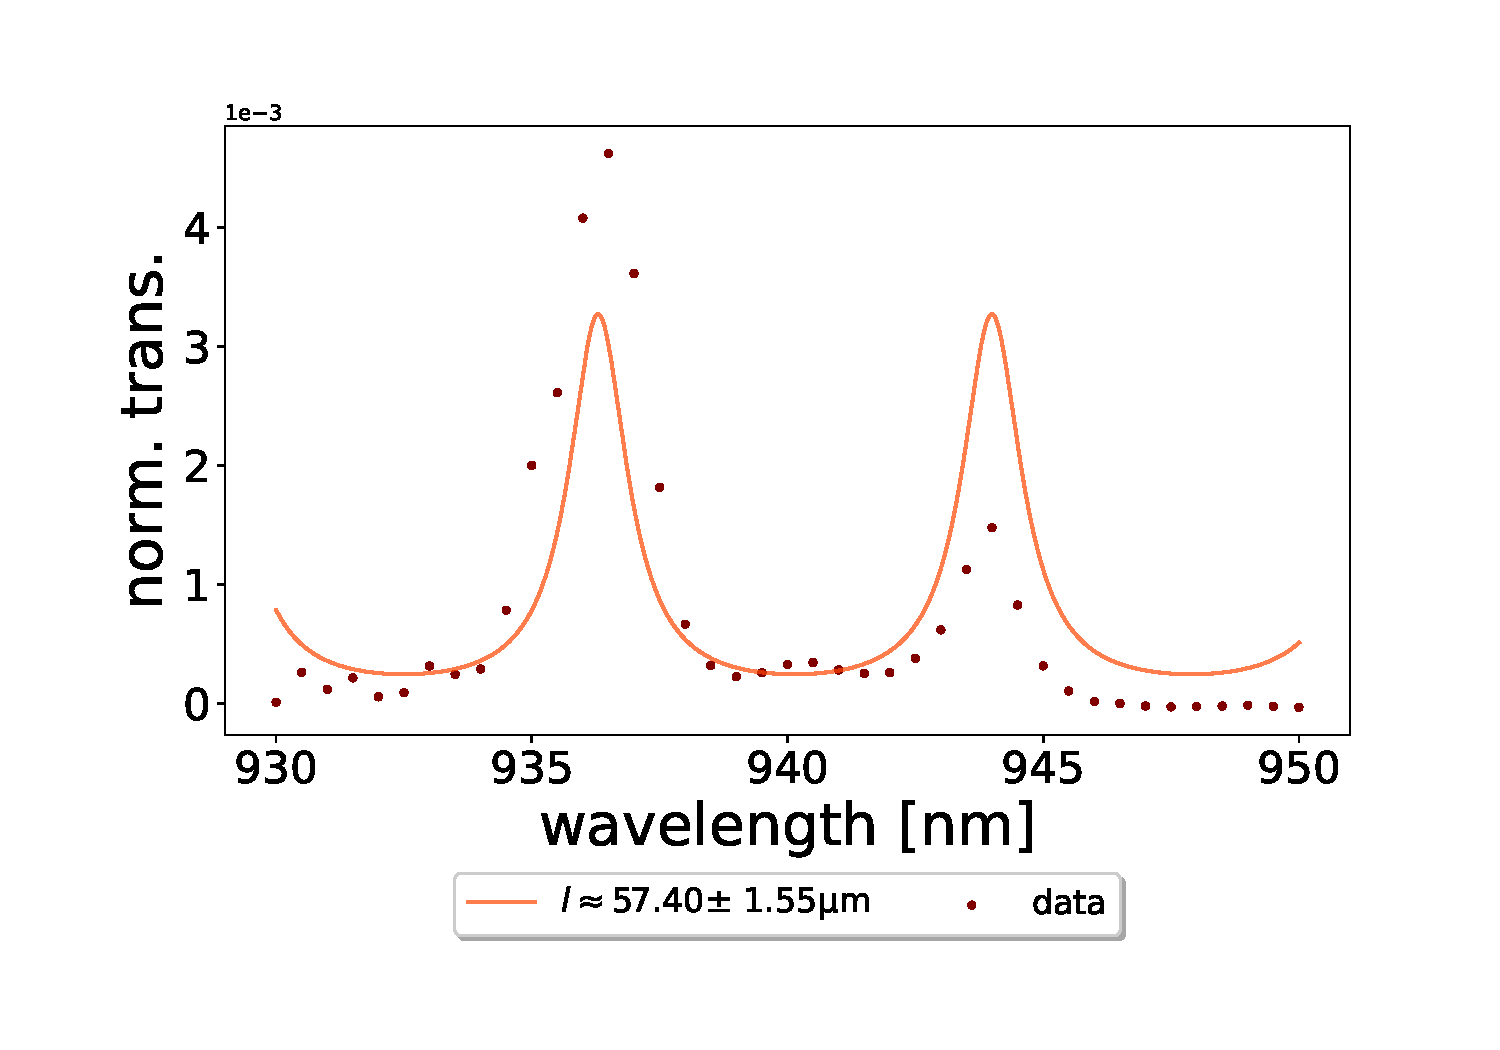
\includegraphics[width=\textwidth]{figures/results/single fano fits/60um_off_res_fabry_perot.pdf}
        \caption{}
        \label{fig:short_single_fano_FSR}
    \end{subfigure}
    \begin{subfigure}[b]{0.49\textwidth}
        \centering
        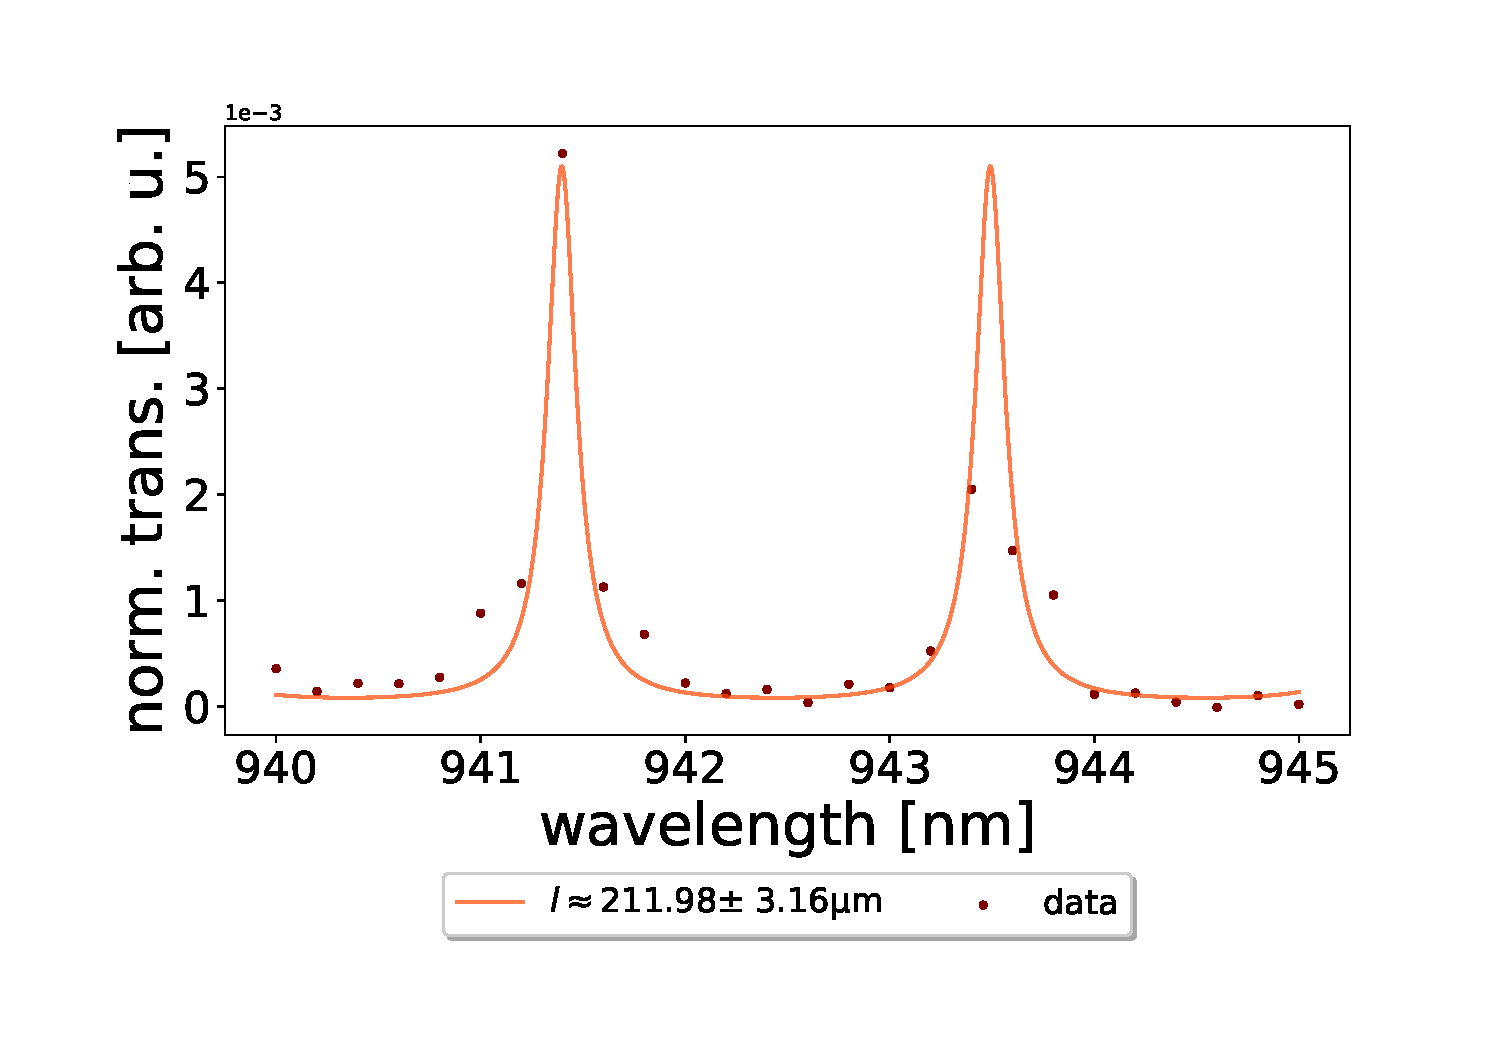
\includegraphics[width=\textwidth]{figures/results/single fano fits/220um_off_res_fabry_perot.pdf}
        \caption{}
        \label{fig:long_single_fano_FSR}
    \end{subfigure}
    \caption{(a) shows an off-resonance wavelength scan of single Fano cavity consisting of a HR broadband mirror and G1 for a cavity length of $l = 57.40 \pm 1.55 \mu m$. (b) shows this for a single Fano cavity of length $l = 211.98 \pm 3.16 \mu m$. Each length is determined from these measurements by measuring the FSR and utilizing that $l = \lambda_0^2/(2\cdot FSR)$.}
    \label{fig:single_fano_fsr_scans}
\end{figure}

Figure \ref{fig:M5/G1_single_fano_trans_examples} shows examples of resonance transmission spectra of the single Fano cavity. The examples are taken for lengths corresponding to the ones found from the off-resonance spectra shown in figure \ref{fig:single_fano_fsr_scans} above. The figures are depicted with each their corresponding least squares fits to the generalized Fano model shown in eq. (\ref{eq:general_fano_model}) in order to determine the linewidth (HWHM) of the profile. The errors of the linewidths are here found from the error of the fit and are mainly used to determine the quality of the measurement. 

\begin{figure}[h!]
    \centering
    \begin{subfigure}[b]{0.49\textwidth}
        \centering
        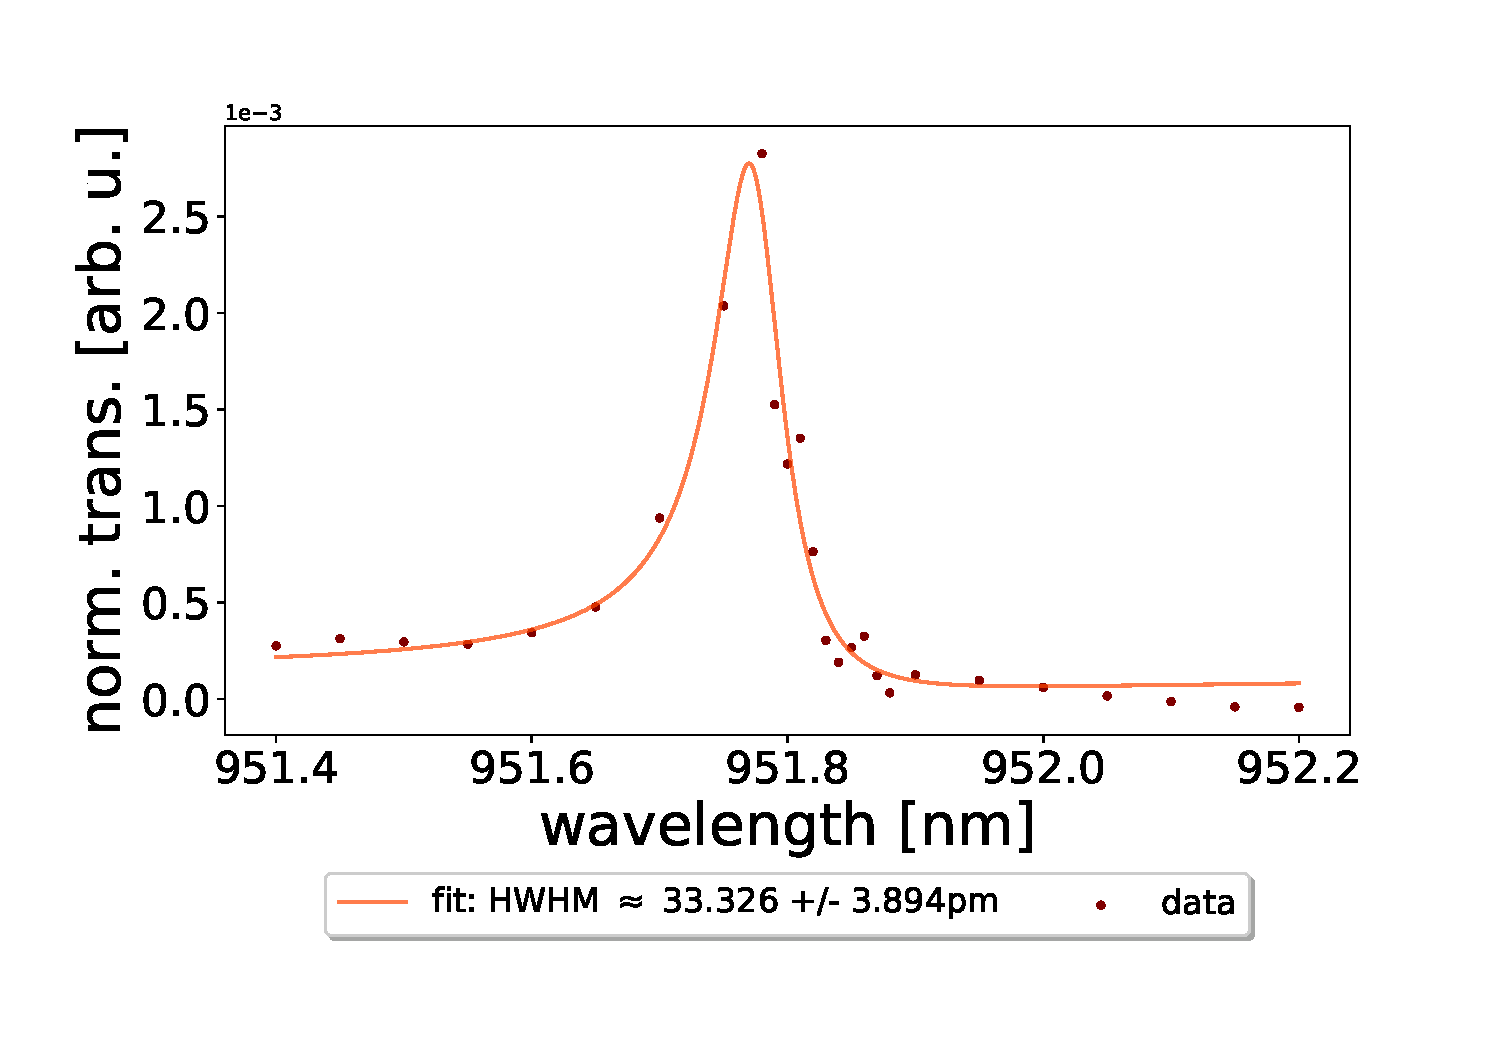
\includegraphics[width=\textwidth]{figures/results/single fano fits/60um_M5_fit_1.pdf}
        \caption{}
        \label{fig:short_single_fano_trans}
    \end{subfigure}
    \begin{subfigure}[b]{0.49\textwidth}
        \centering
        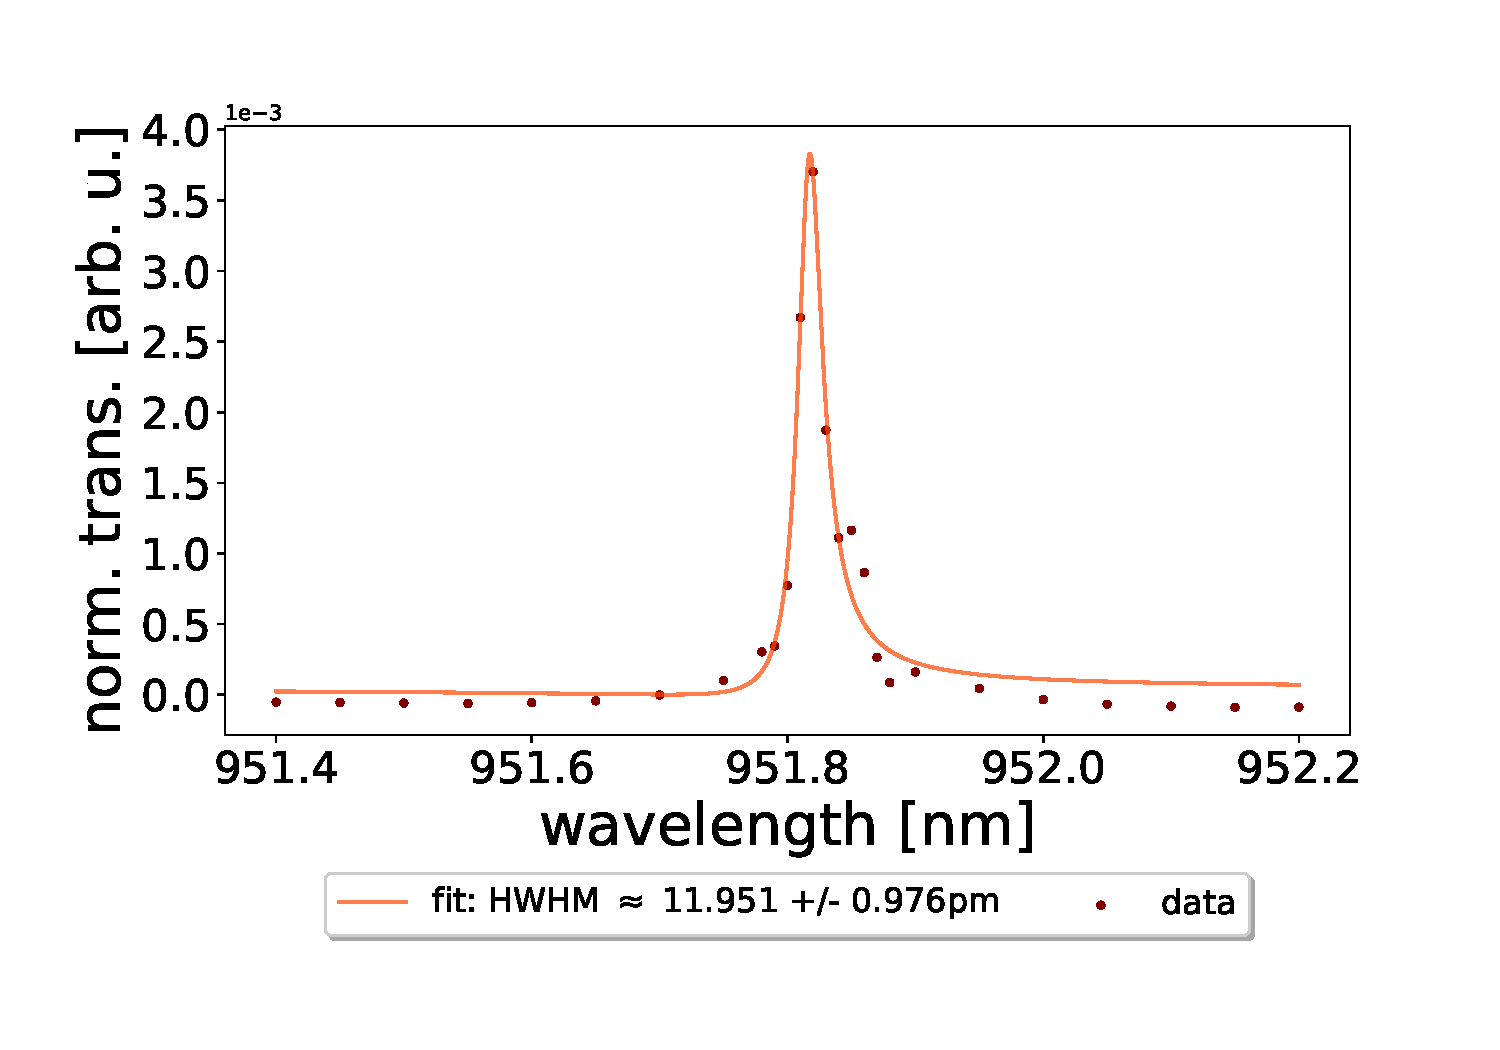
\includegraphics[width=\textwidth]{figures/results/single fano fits/220um_M5_fit_4.pdf}
        \caption{}
        \label{fig:long_single_fano_trans}
    \end{subfigure}
    \caption{Single Fano resonance transmission profiles of a cavity consisting of a HR broadband mirror of reflectvitiy $R=99.7\%$ and Fano mirror G1. (a) shows the profile of a cavity of length $l = 57.40 \pm 1.55 \mu m$ and displays a linewidth of $HWHM = 33.907 \pm 3.838$pm. (b) shows the profile of a cavity of length $l = 211.98 \pm 3.16 \mu m$, with a linewidth of $HWHM = 11.982 \pm 0.964$pm.}
    \label{fig:M5/G1_single_fano_trans_examples}
\end{figure}

At each cavity length, the resonance transmission profile was recorded a number of times and the average value was taken to be the true found value of the linewidth. Figure \ref{fig:HWHM_vs_length_single_fano_data} shows the result of a measurement series consisting of five cavity lengths approximately ranging from $20\mu m \leq l \leq 400 \mu m$, where the error of each measurement is given as the standard deviation of the values of all measurements recorded at each cavity length\cite{Hughes}. The error depicted in the x-direction is found from the error of the fit of the Fabry-Perot transmission function to the off-resonance spectra. The blue dashed line indicates the linewidth of a broadband cavity of similar losses according to eq. (\ref{eq:analytical_linewidth_broadband}) and the orange dashed line indicates the analytical linewidth of the single Fano cavity considered consisting of G1 and the HR broadband mirror estimated using eq. (\ref{eq:analytical_linewidth_single_fano}). The black points are linewidths found by fitting single Fano transmission profiles simulated using eq. (\ref{eq:single_fano_trans}) to the generalized Fano model in eq. (\ref{eq:general_fano_model}) for comparison. 

It is seen that the analytical model, the simulated linewidths and the measured linewidths coincide very well for the cavity lengths that are well within the Fano regime and deviates slightly for longer lengths. This trend agrees nicely with what has previously been found for the single Fano cavity transmission\cite{Mitra} and is likely a consequence of the very narrow linewidths of the cavity in the standard regime, as this increases the sensitivity to any noise regarding the cavity length, e.g. mechanical vibrations in the setup.

\begin{figure}[h!]
    \centering
    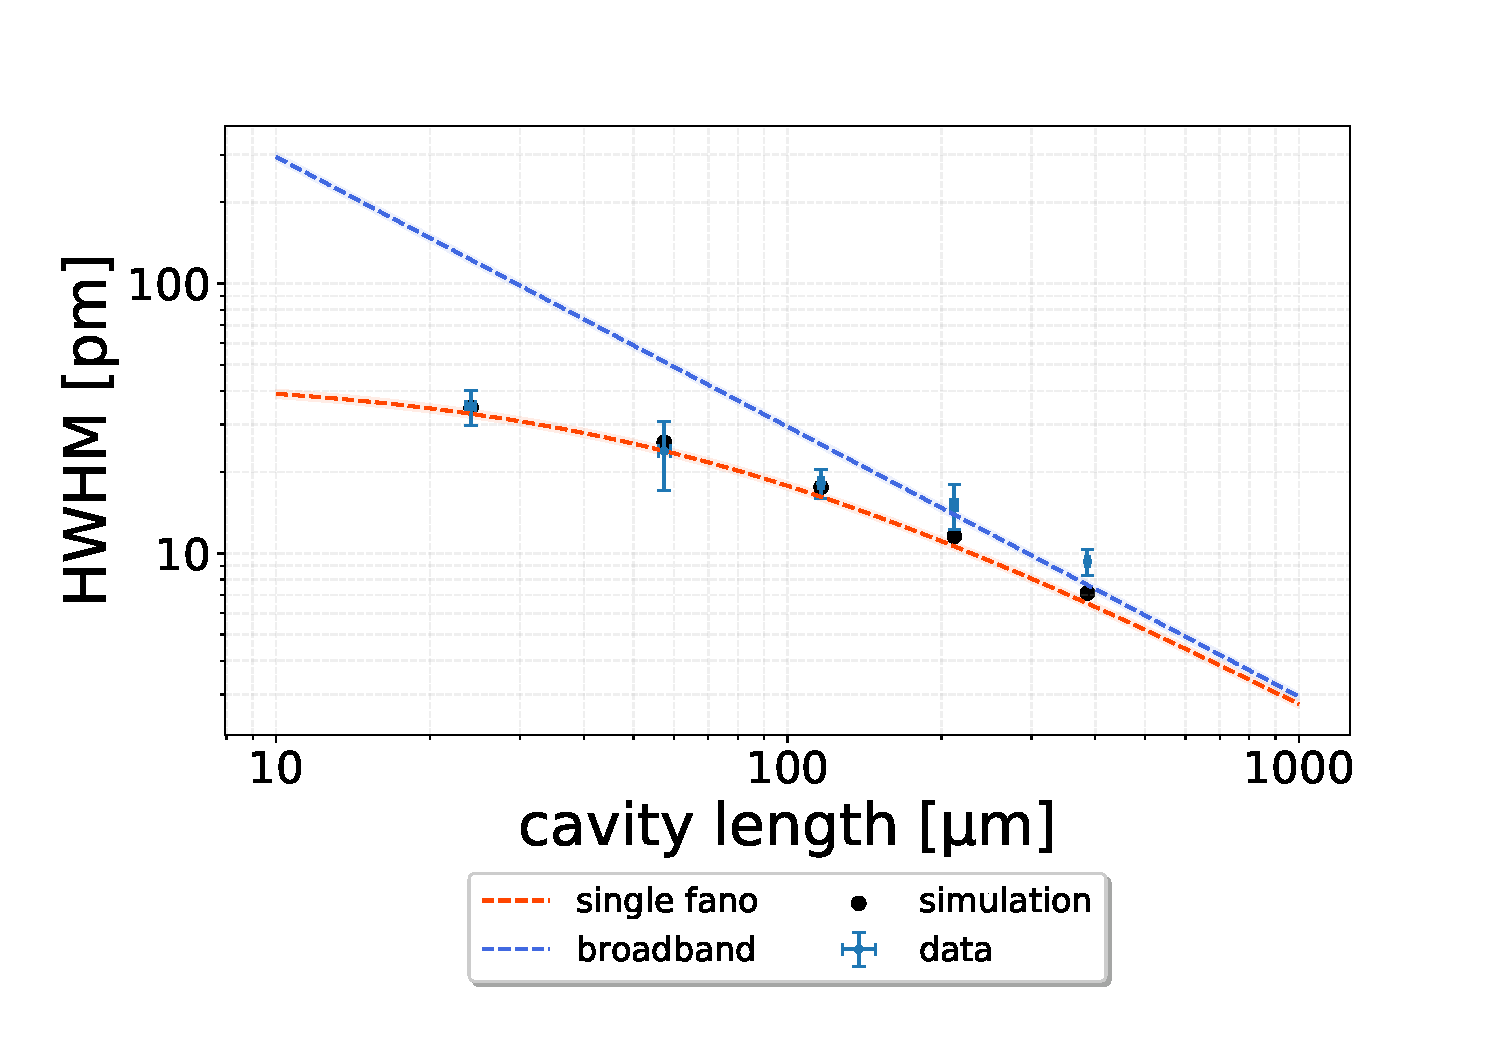
\includegraphics[width=0.7\textwidth]{figures/results/HWHM_vs_cavity_length_single_fano.pdf}
    \caption{The linewidth (HWHM) as a function of resonant cavity length. The blue dashed line indicates the analytical linewidth for a broadband cavity, and the orange dashed line shows the corresponding analytical linewidth for a single Fano cavity of similar losses to the one realized experimentally. The blue points and corresponding errorbars shows the measured linewidths found as averages of all recorded values at each length and the error is found as the standard deviation of these values. The black points are the linewidths of simulated spectra. The spectra used to determine the points depicted can be found in Appendix \ref{appendix:Measured single Fano transmission data}.}
    \label{fig:HWHM_vs_length_single_fano_data}
\end{figure}

\newpage
\subsection{The double Fano cavity}\label{sec:the_double_fano_cavity_results}

In this section I will present of the results for the characterization of a double Fano cavity consisting of Fano mirrors G1 and G2. First we examine the simulated spectra of the double Fano transmission intensity profile as a function of the incident wavelength simulated with the parameters for G1 given in eq. (\ref{eq:G1_params}) and for G2 given in eq. (\ref{eq:G2_params}). Figures \ref{fig:G1_and_G2_full_range_spectra} and \ref{fig:G1_and_G2_short_range_spectra} shows the simulated spectra for cavity lengths according to $l=l_{G1}$, $l=l_{G2}$ and $l=(l_{G1}+l_{G2})/2$ together with the reflection spectra for G1 and G2 also shown in figure \ref{fig:G1_and_G2_spectral_comparison}. 

\begin{figure}[h!]
    \centering
    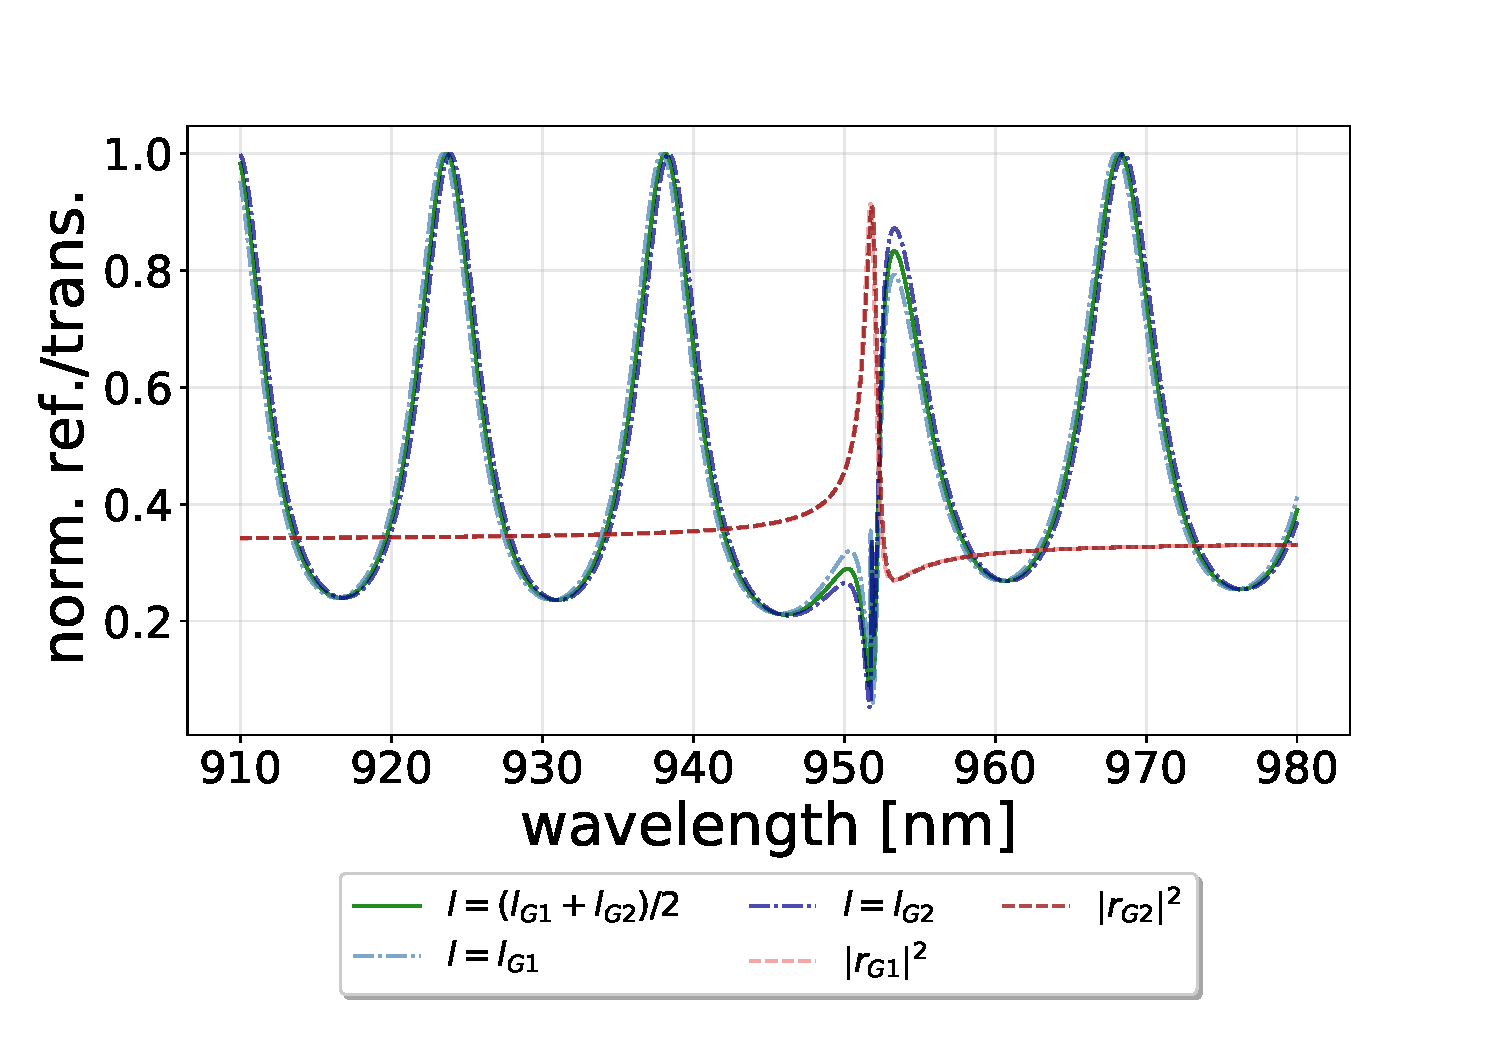
\includegraphics[width=0.7\textwidth]{figures/results/M3:M5/M3:M5_sim_spectra_long.pdf}
    \caption{The simulated spectra of a double Fano cavity consisting of G1 and G2 for lengths $l=l_{G1}$, $l=l_{G2}$ and $l = (l_{G1}+l_{G2})/2$. The two red dashed lines are the normalized reflectivity intensities of G1 and G2, respectively, shown in figure \ref{fig:G1_and_G2_spectral_comparison}. The range plotted is chosen as it resembles the tunable range of the Toptica laser used for the experiments of this project.}
    \label{fig:G1_and_G2_full_range_spectra}
\end{figure}

It is seen in figure \ref{fig:G1_and_G2_full_range_spectra} that the off-resonance level is expected to almost reach unity for a perfectly aligned cavity, for the given direct transmission/reflection coefficient amplitudes $t_d$, $t_d^{\prime}$ and $r_d$, $r_d^{\prime}$. This result for the simulated spectra is indicative of the validity of the assumption that these are approximately identical meaning that $t_{d,G1} \approx t_{d,G2}$ and $r_{d,G1} \approx r_{d,G2}$. Furthermore, the background perfectly resembles a low finesse Fabry-Perot cavity, as is expected from the theory. 

Figure \ref{fig:G1_and_G2_short_range_spectra} shows the transmission spectra of the double Fano cavity zoomed on the resonance wavelengths considered according to the depicted cavity lengths. Here it is seen how the transmission peak at resonance is expected to shift with the cavity length, and that the estimated detuning $\Delta$ of the two Fano mirrors seems to be sufficiently small to realize the double Fano resonance profile. Lastly, it is seen what to expect in terms of the peak height of the resonance profile as this is an important merit when practically estimating the losses, and by extension the alignment, of the cavity in the lab. 

\begin{figure}[h!]
    \centering
    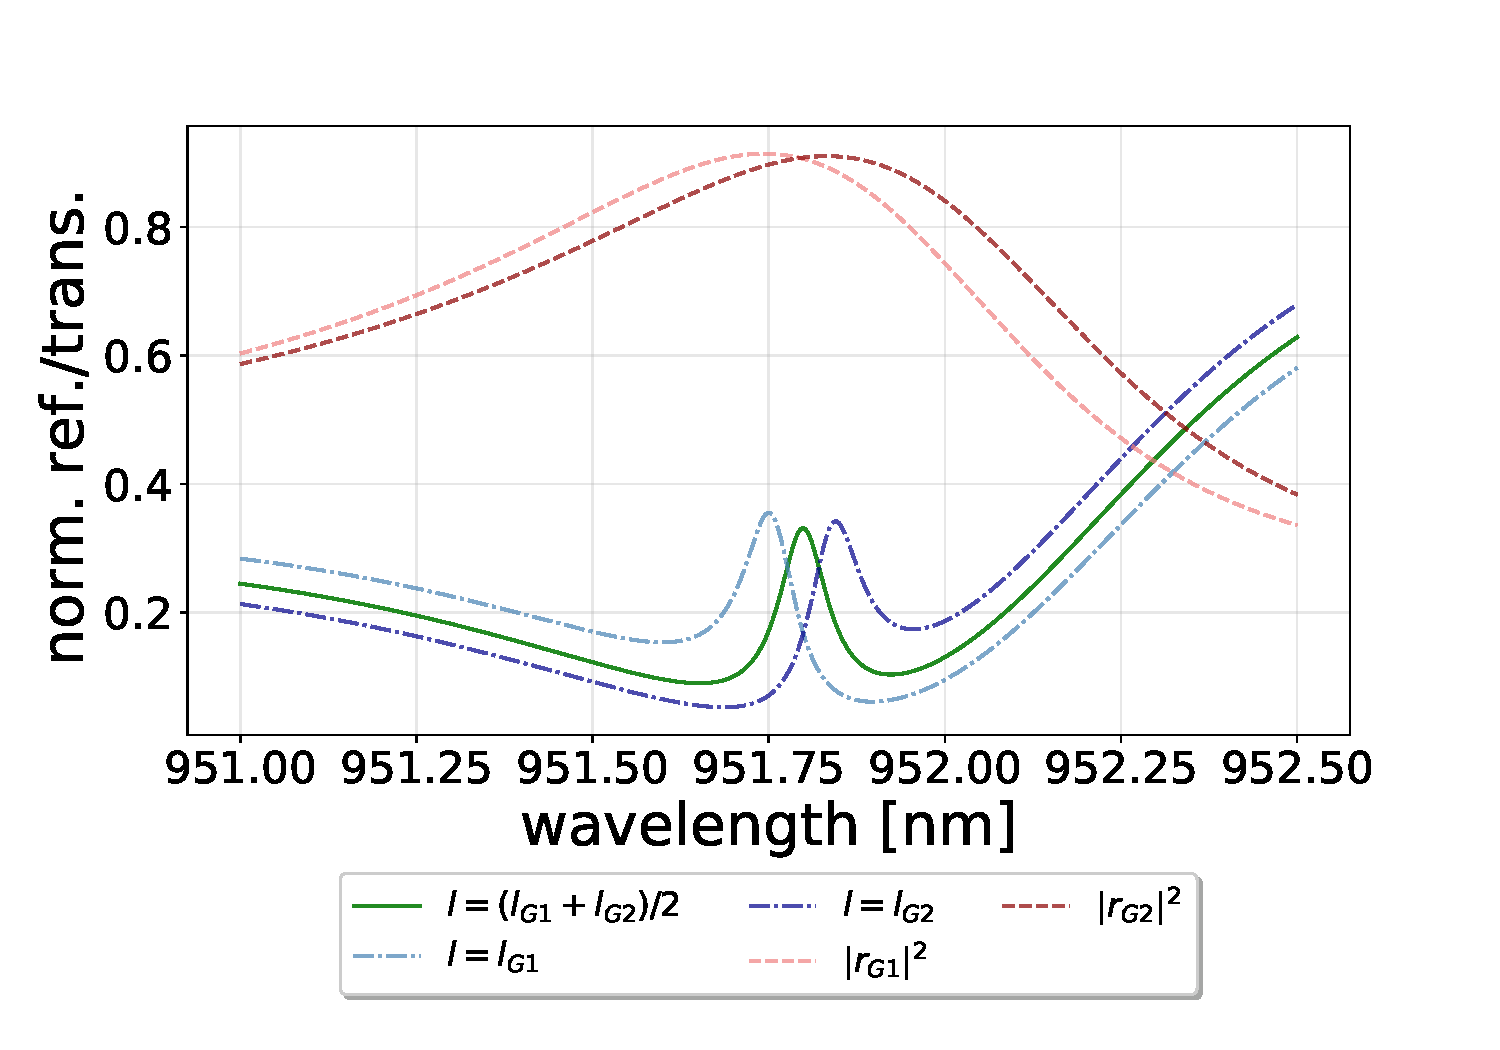
\includegraphics[width=0.7\textwidth]{figures/results/M3:M5/M3:M5_sim_spectra_short.pdf}
    \caption{The simulated spectra of a double Fano cavity consisting of G1 and G2 for lengths $l=l_{G1}$, $l=l_{G2}$ and $l = (l_{G1}+l_{G2})/2$ focused around the corresponding resonance wavelengths. The two red dashed lines are the normalized reflection intensities of G1 and G2, respectively. These are shown in figure \ref{fig:G1_and_G2_spectral_comparison}.}
    \label{fig:G1_and_G2_short_range_spectra}
\end{figure}

The transmission profile for different cavity length where simulated in order to determine the optimal value. Figure \ref{fig:G1_G2_cmap} shows a colormap of the resonance profile as a function of wavelength and cavity length ranging $l_{G1} \leq l \leq l_{G2}$. The signal intensity is indicated by the brightness of the colormap, such that the resonance wavelength and cavity length is indicated by the "line" showing the resonance peak moving in terms of both parameters. 

\begin{figure}[h!]
    \centering
    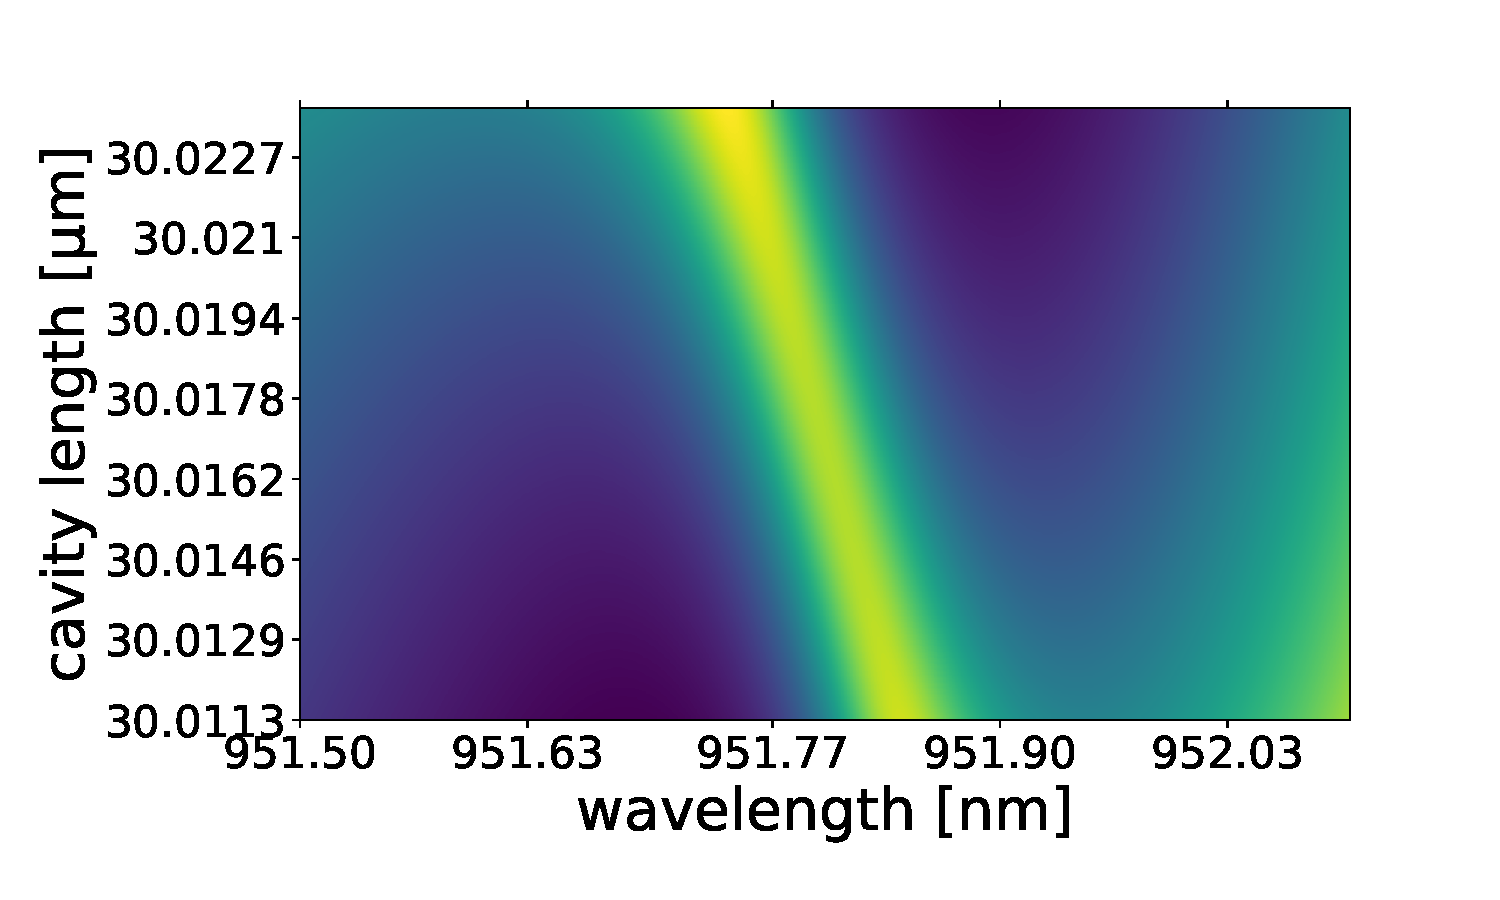
\includegraphics[width=0.7\textwidth]{figures/results/M3:M5/G1:G2_cmap.pdf}
    \caption{Colormap of the resonance transmission profile of the double Fano cavity consisting of G1 and G2. The brightness of the colormap indicates the intensity/peak height while the varied parameters are the wavelength and cavity length ranging $l_{G1} \leq l \leq l_{G2}$.}
    \label{fig:G1_G2_cmap}
\end{figure}

The colormap provides a qualitative and intuitive image of the behaviour of the double Fano transmission profile, but the optimal cavity length to optimize with respect to the linewidth is nearly impossible to determine from this alone. Figure \ref{fig:G1/G2_lw_vs_cavity_length} instead shows the linewidth of intracavity spectra as a function of the cavity length and shows that the optimal cavity length is approximately given as $l \approx (l_{G1} + l_{G2})/2$. In reality, the assymetric structure of the Fano mirror spectra results in an exact answer to the optimal cavity length that is more complicated, and likely impossible to realize in the lab. For this reason the approximate interpretation of the cavity length analysis is sufficient for practical purposes.

\begin{figure}[h!]
    \centering
    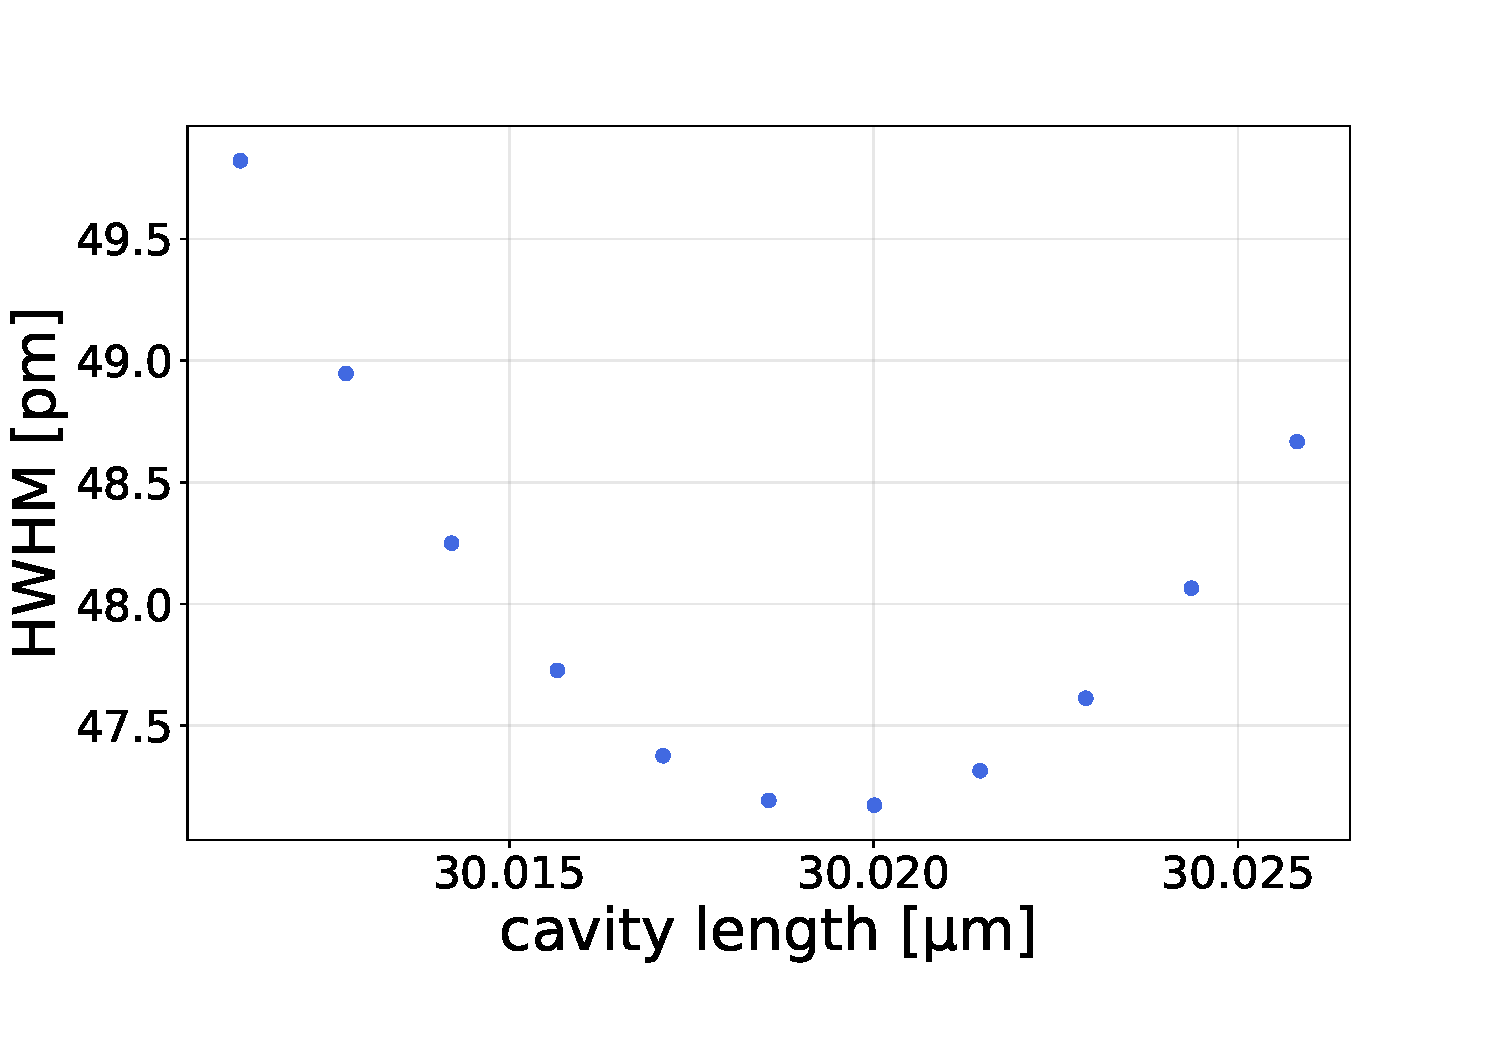
\includegraphics[width=0.7\textwidth]{figures/results/M3:M5/M3:M5_lw_vs_length.pdf}
    \caption{The simulated intracavity linewidth as a function of cavity length ranging $l_{G1} \leq l \leq l_{G2}$. Each linewidth is found by fitting simulated spectra to the generalized Fano model in eq. (\ref{eq:general_fano_model}).}
    \label{fig:G1/G2_lw_vs_cavity_length}
\end{figure}

\newpage
\subsubsection{Realizing the double fano model}\label{sec:realizing_the_double_fano_model}

To realize the double Fano model in a satisfying way a relatively broad spectrum is examined as the off-resonance profile resembling a low-finesse Fabry-Perot transmission spectrum, with near-unity transmission levels at each Fabry-Perot resonance peak, is considered a defining feature of the double Fano cavity. In this section I will present three spectra obtained experimentally and compared with corresponding simulated spectra for lengths $l=l_{G1}$, $l=l_{G2}$ and $l=(l_{G1} + l_{G2})/2$. Furthermore, I present the same experimental spectra fitted to the double Fano cavity transmission model with varied fitting parameters. The first two spectra presented have been fitted with fitting parameters given by $\lambda_{0,G1}$, $\lambda_{1,G1}$, $\lambda_{0,G2}$, $\lambda_{1,G2}$, $l$ and $L$, where $l$ is the cavity length and $L = 1-|r|^2$ is the cavity losses. The last spectrum presented proved unable to agree well with the model given the aforementioned fitting parameters, and for this reason all Fano mirror parameters for both G1 and G2 are considered variable in this fit along with the cavity length $l$ and cavity losses $L$.

\begin{figure}[h!]
    \centering
    \begin{subfigure}[b]{0.49\textwidth}
        \centering
        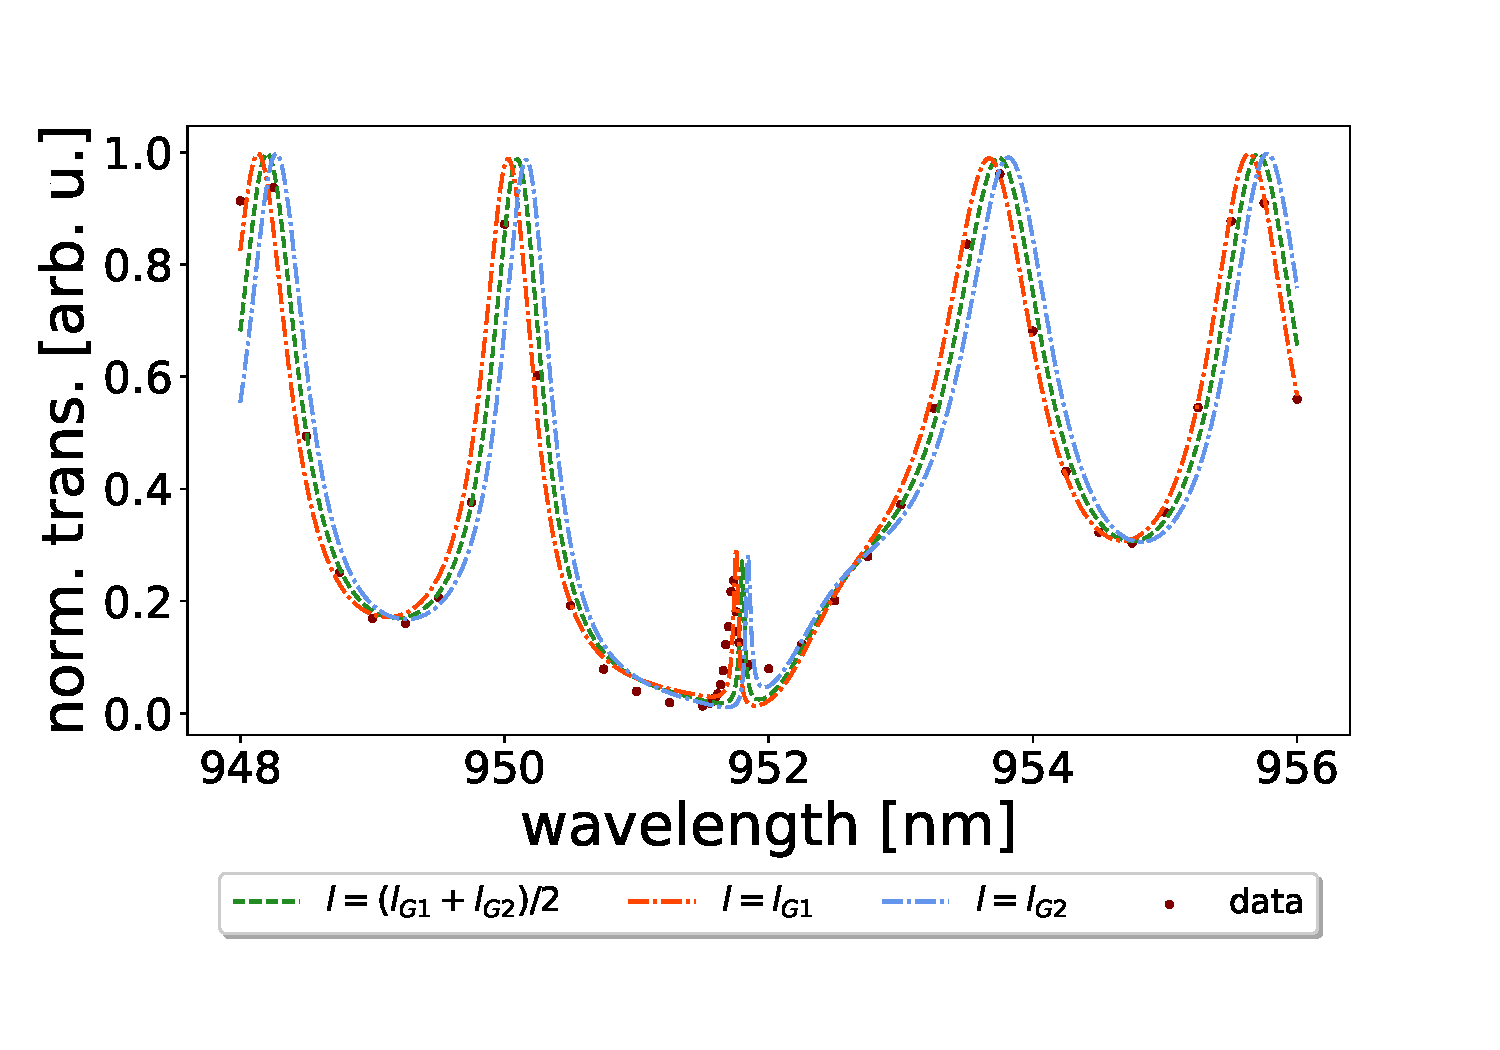
\includegraphics[width=\textwidth]{figures/results/238um_long_scan_sim_comparison.pdf}
        \caption{}
        \label{fig:238um_long_scan_sim_comparison}
    \end{subfigure}
    \begin{subfigure}[b]{0.49\textwidth}
        \centering
        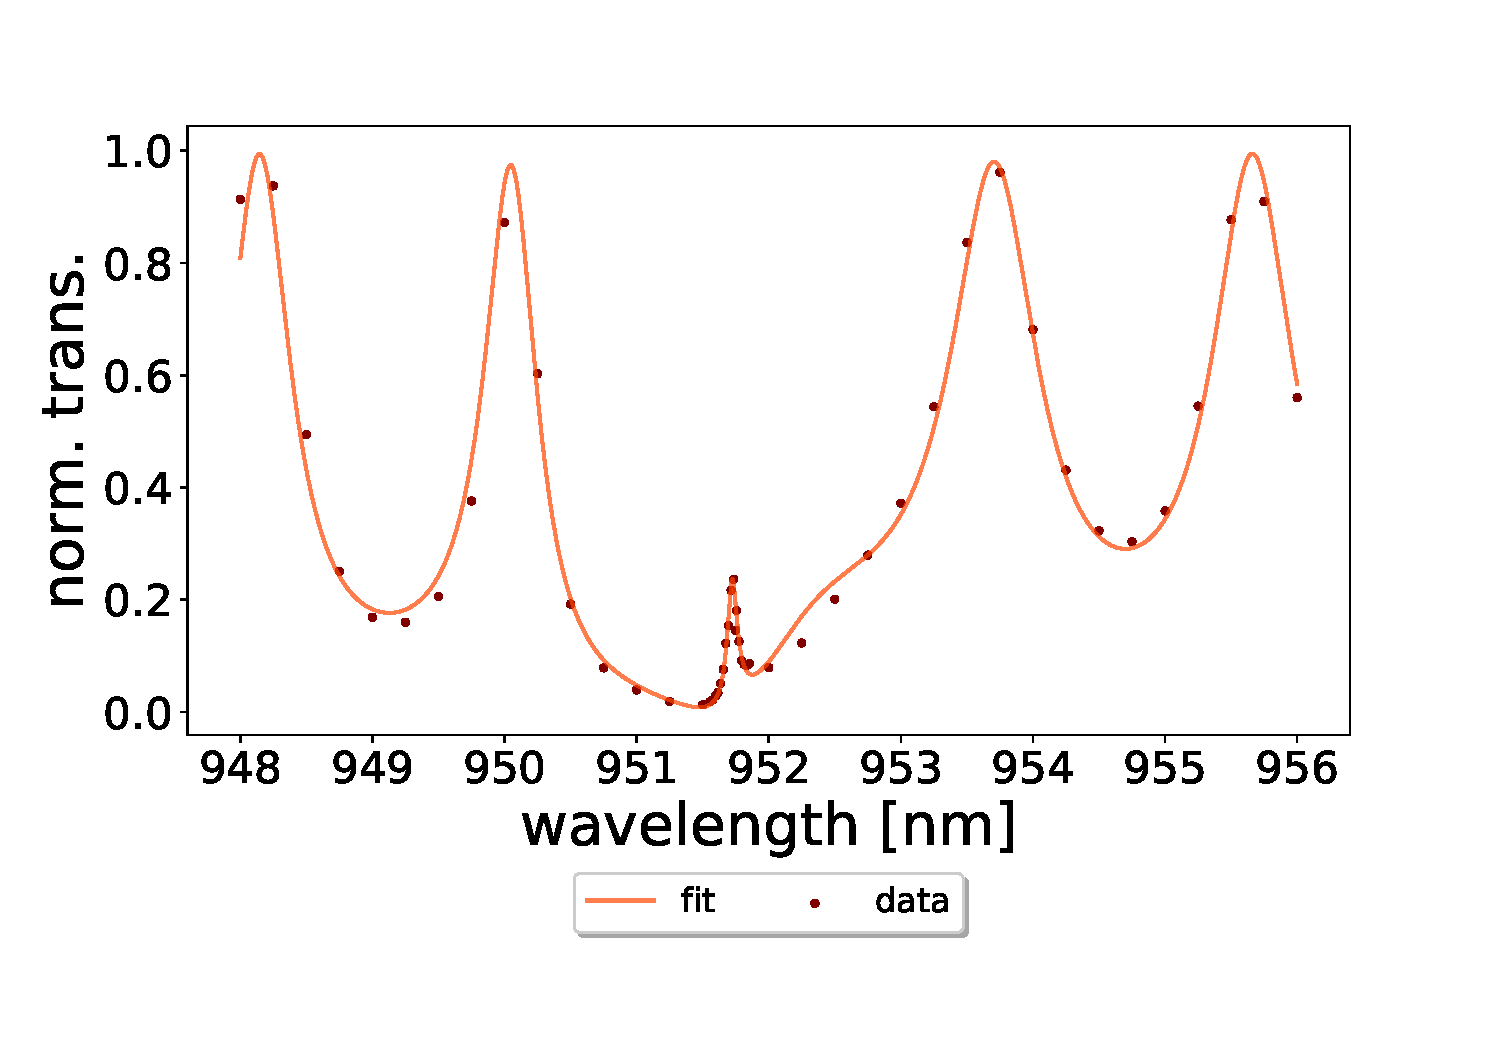
\includegraphics[width=\textwidth]{figures/results/238um_long_scan_fit2.pdf}
        \caption{}
        \label{fig:238um_long_scan_fit}
    \end{subfigure}
    \caption{(a) shows recorded data of the double Fano cavity transmission compared with simulated spectra for cavity lengths of $l_{G1} = 239.3975 \mu m$, $l_{G2} = 239.4317 \mu m$ and $(l_{G1} + l_{G2})/2 = 239.4146 \mu m$. (b) shows a least squares fit of the recorded data to the double Fano cavity transmission model in eq. (\ref{eq:double_fano_transmission}).}
    \label{fig:238um_cavity_fit_and_sim}
\end{figure}

\newpage
Figure \ref{fig:238um_long_scan_sim_comparison} show the comparison of data and simulation for a cavity of lengths given as $l_{G1} = 239.3975 \mu m$, $l_{G2} = 239.4317 \mu m$ and $(l_{G1} + l_{G2})/2 = 239.4146 \mu m$. Figure \ref{fig:238um_long_scan_fit} shows a least squares fit of the recorded data to the double Fano transmission function with fitting parameters found as 
\begin{equation}
    \lambda_{0,G1} = 951.509 \pm 0.036 \text{nm}, \:\: \lambda_{1,G1} = 951.586 \pm 0.107 \text{nm}
\end{equation}

for Fano mirror G1,

\begin{equation}
    \lambda_{0,G2} = 951.782 \pm 0.041 \text{nm}, \:\: \lambda_{1,G2} = 951.934 \pm 0.058 \text{nm}
\end{equation}

for Fano mirror G2, and

\begin{equation}
    l = 238.925 \pm 0.002 \mu m, \:\: L = 0.178 \pm 0.038
\end{equation}
for the cavity length and losses.

\begin{figure}[h!]
    \centering
    \begin{subfigure}[b]{0.49\textwidth}
        \centering
        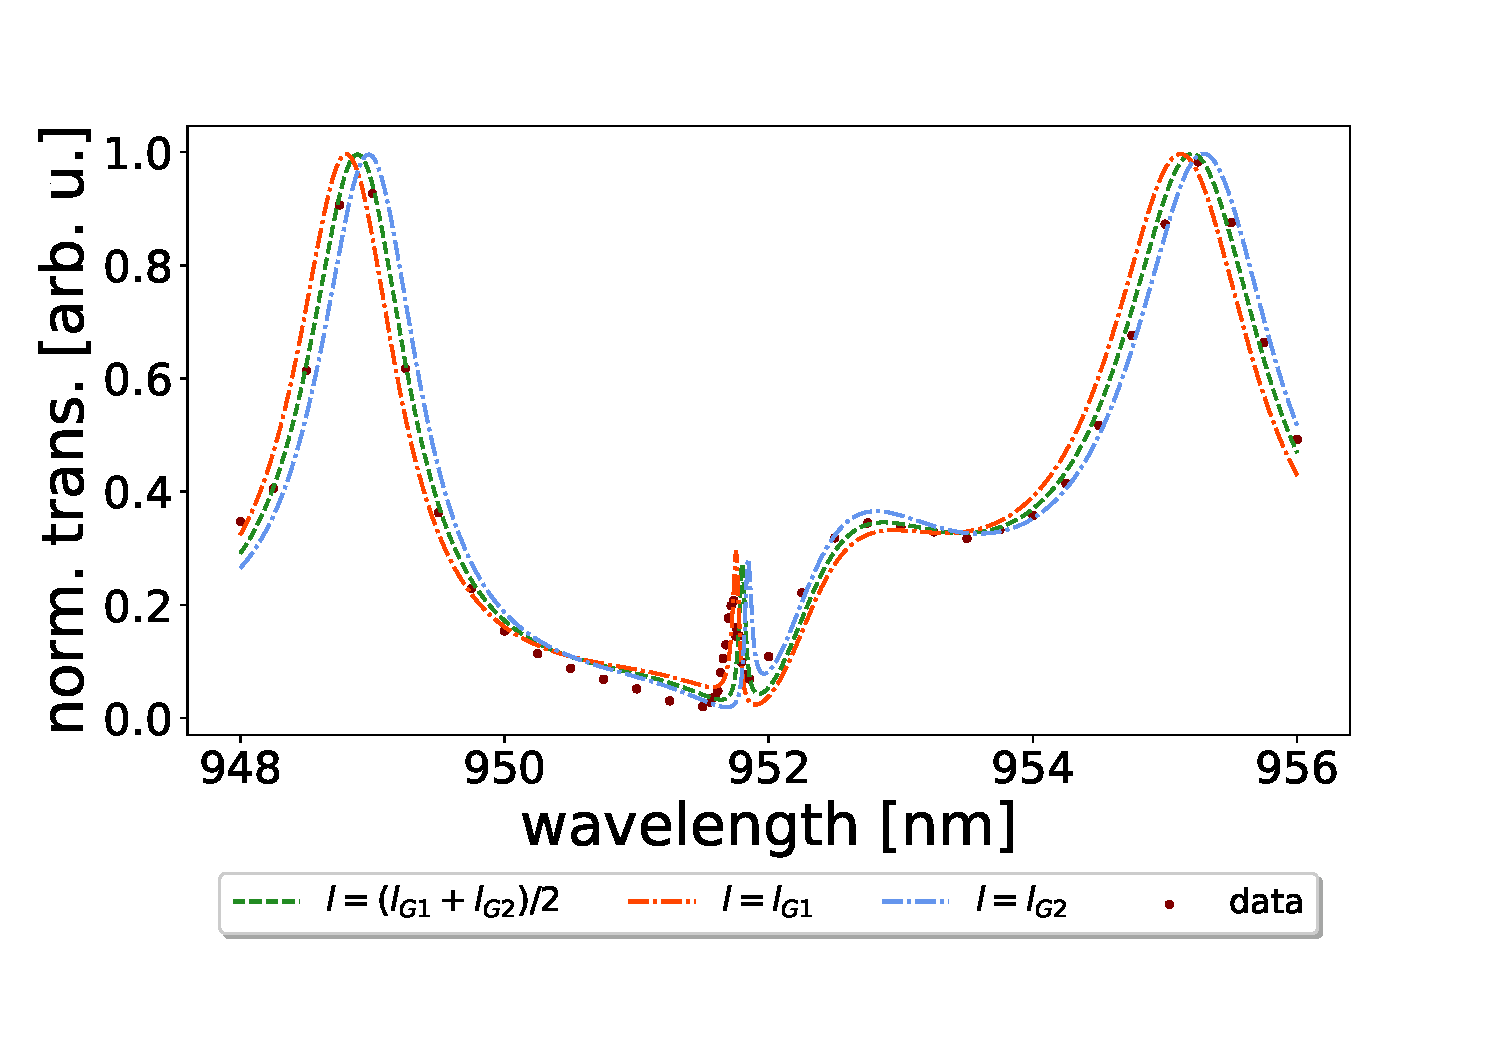
\includegraphics[width=\textwidth]{figures/results/129um_long_scan_sim_comparison.pdf}
        \caption{}
        \label{fig:129um_long_scan_sim_comparison}
    \end{subfigure}
    \begin{subfigure}[b]{0.49\textwidth}
        \centering
        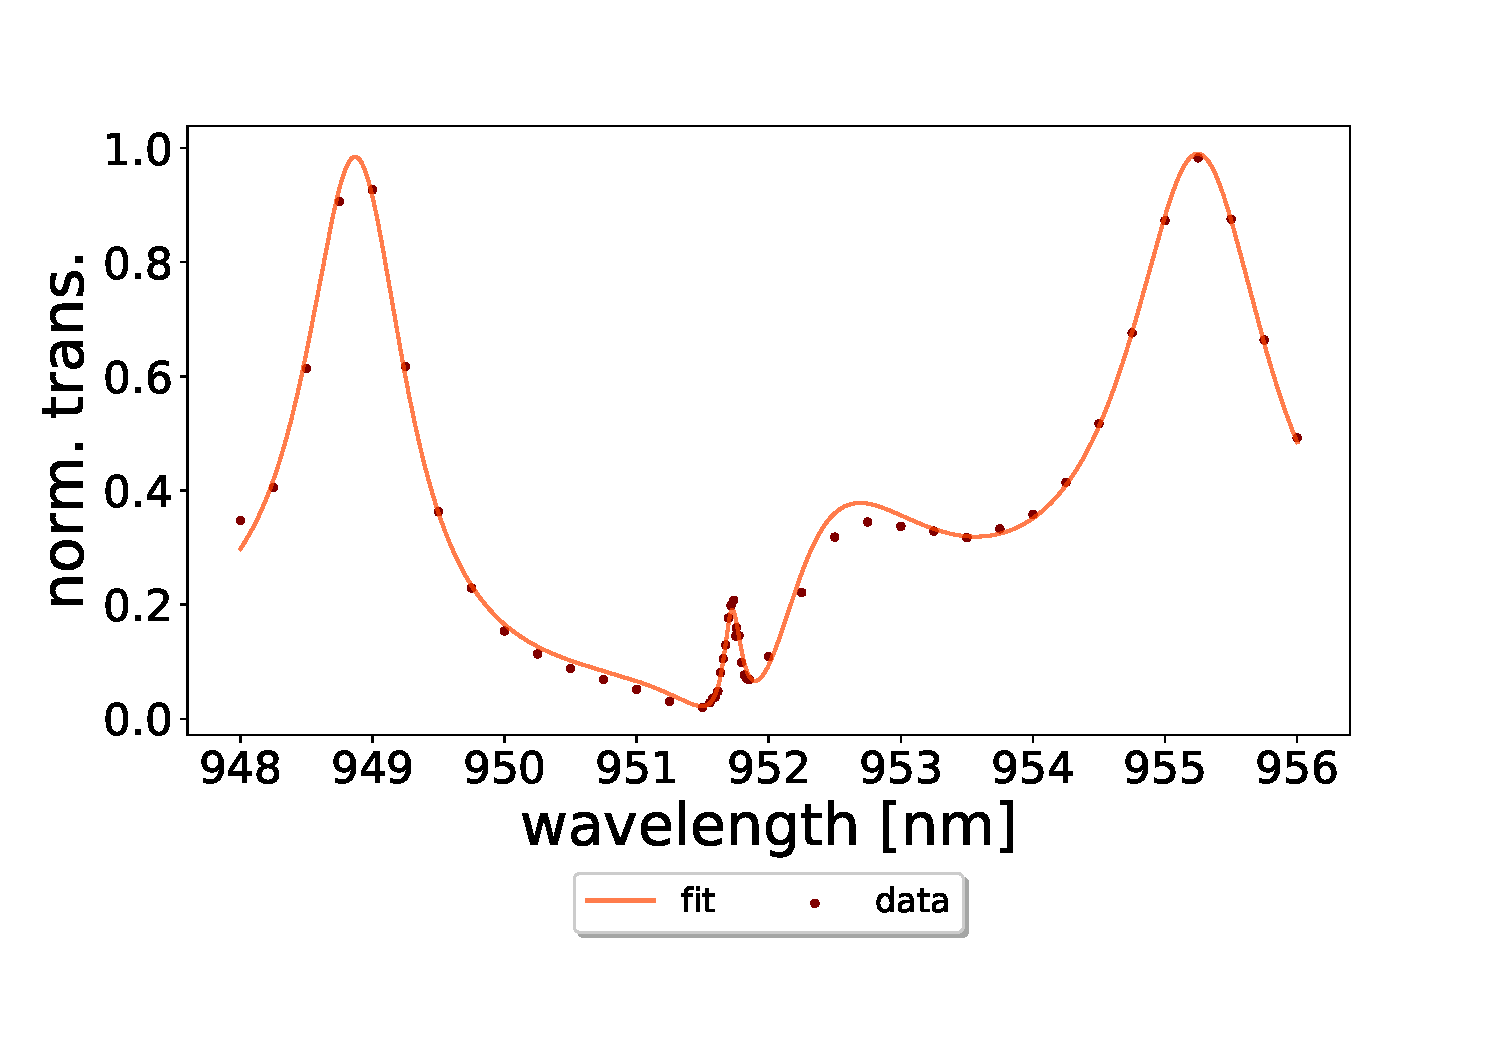
\includegraphics[width=\textwidth]{figures/results/129um_long_scan_fit2.pdf}
        \caption{}
        \label{fig:129um_long_scan_fit}
    \end{subfigure}
    \caption{(a) shows recorded data of the double Fano cavity transmission compared with simulated spectra for cavity lengths of $l_{G1} = 140.4152 \mu m$, $l_{G2} = 140.4401 \mu m$ and $(l_{G1} + l_{G2})/2 = 140.4277 \mu m$. (b) shows a least squares fit of the recorded data to the double Fano cavity transmission model in eq. (\ref{eq:double_fano_transmission}).}
    \label{fig:129um_cavity_fit_and_sim}
\end{figure}

\newpage
Figure \ref{fig:129um_long_scan_sim_comparison} shows the comparison of data and simulation for a cavity of lengths given as $l_{G1} = 140.4152 \mu m$, $l_{G2} = 140.4401 \mu m$ and $(l_{G1} + l_{G2})/2 = 140.4277 \mu m$. Figure \ref{fig:129um_long_scan_fit} shows a least squares fit of the recorded data to the double Fano transmission function with fitting parameters found as 

\begin{equation}
    \lambda_{0,G1} = 951.546 \pm 0.015 \text{nm}, \:\: \lambda_{1,G1} = 951.719 \pm 0.040 \text{nm}
\end{equation}

for Fano mirror G1,

\begin{equation}
    \lambda_{0,G2} = 951.868 \pm 0.016 \text{nm}, \:\: \lambda_{1,G2} = 951.963 \pm 0.039 \text{nm}
\end{equation}

for Fano mirror G2, and

\begin{equation}
    l = 139.953 \pm 0.001 \mu m, \:\: L = 0.293 \pm 0.033
\end{equation}

for the cavity length and losses.

The additional optical parameters for G1 and G2, $t_d$, $\gamma_{\lambda}$ and $\beta$, are kept constant for the cavities of lengths $l\approx 239 \mu m$ and $l \approx 139 \mu m$, and are thus given in eqs. (\ref{eq:G1_params}) and (\ref{eq:G2_params}). The choice of fixed and variable parameters in the least squares fit is justificed by the angular dependence of the guided-mode resonance wavelength outlined in \cite{Parthenopoulos}. It is hence evident that $\lambda_0$ and $\lambda_1$ potentially shifts slightly for different measurements and is for this reason denoted a variable fitting parameter. The additional optical parameters mentioned above have shown to be constant, even for slight misalignments, and are therefore rightly fixed when fitting. 

\begin{figure}[h!]
    \centering
    \begin{subfigure}[b]{0.49\textwidth}
        \centering
        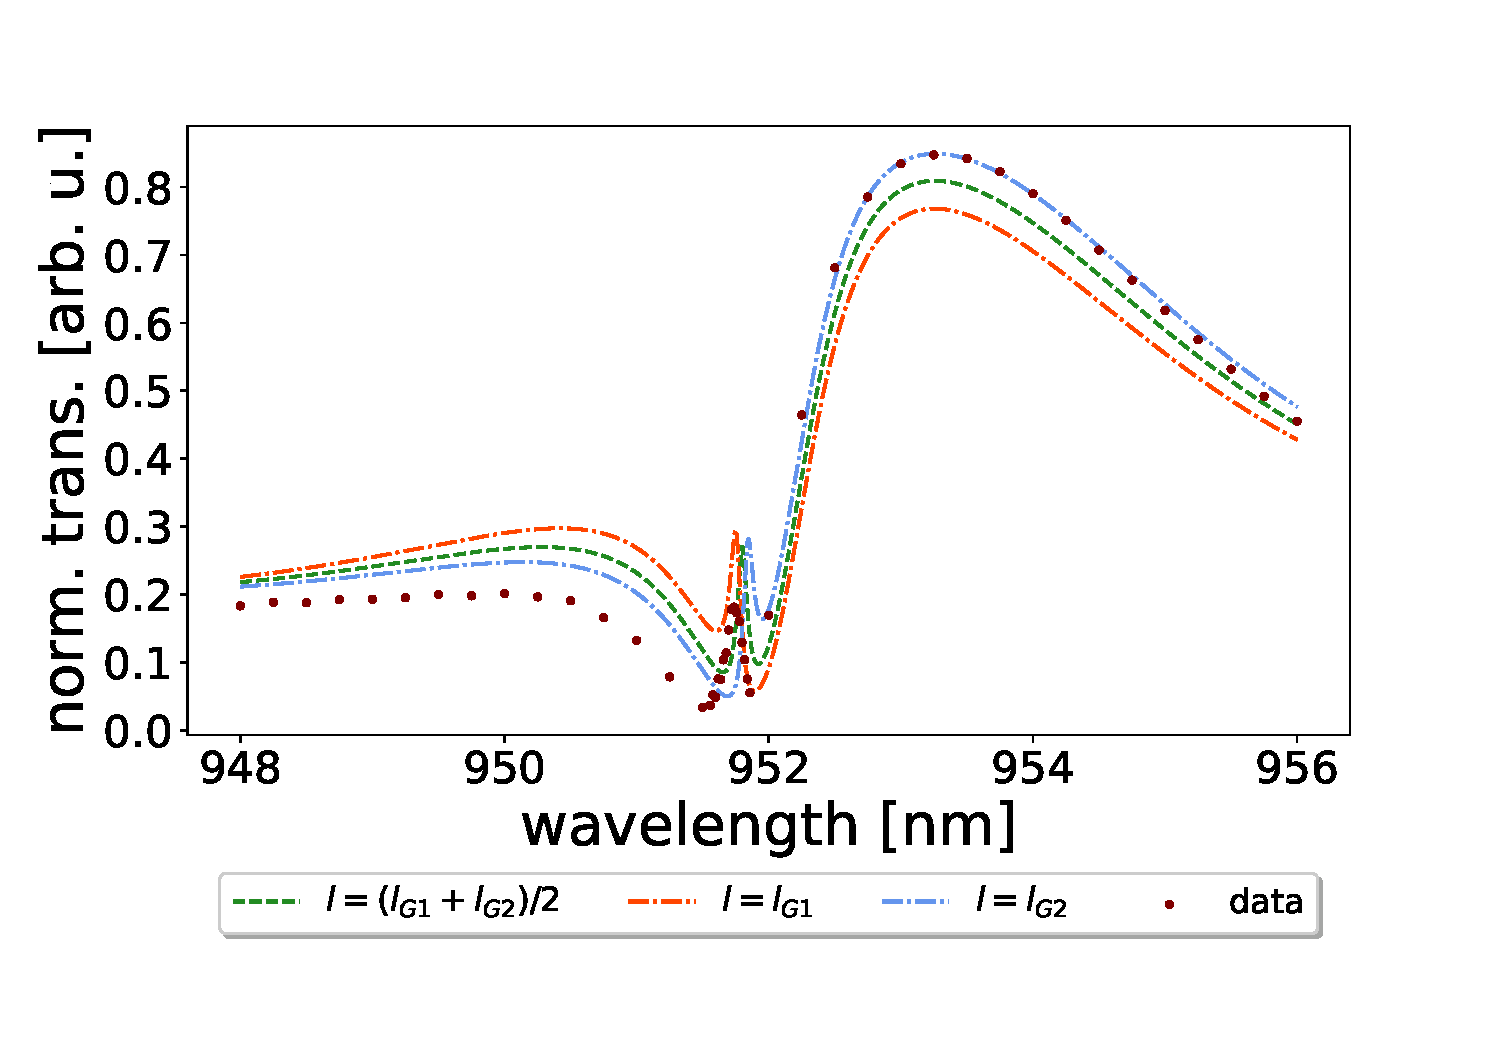
\includegraphics[width=\textwidth]{figures/results/34um_long_scan_sim_comparison.pdf}
        \caption{}
        \label{fig:34um_long_scan_sim_comparison}
    \end{subfigure}
    \begin{subfigure}[b]{0.49\textwidth}
        \centering
        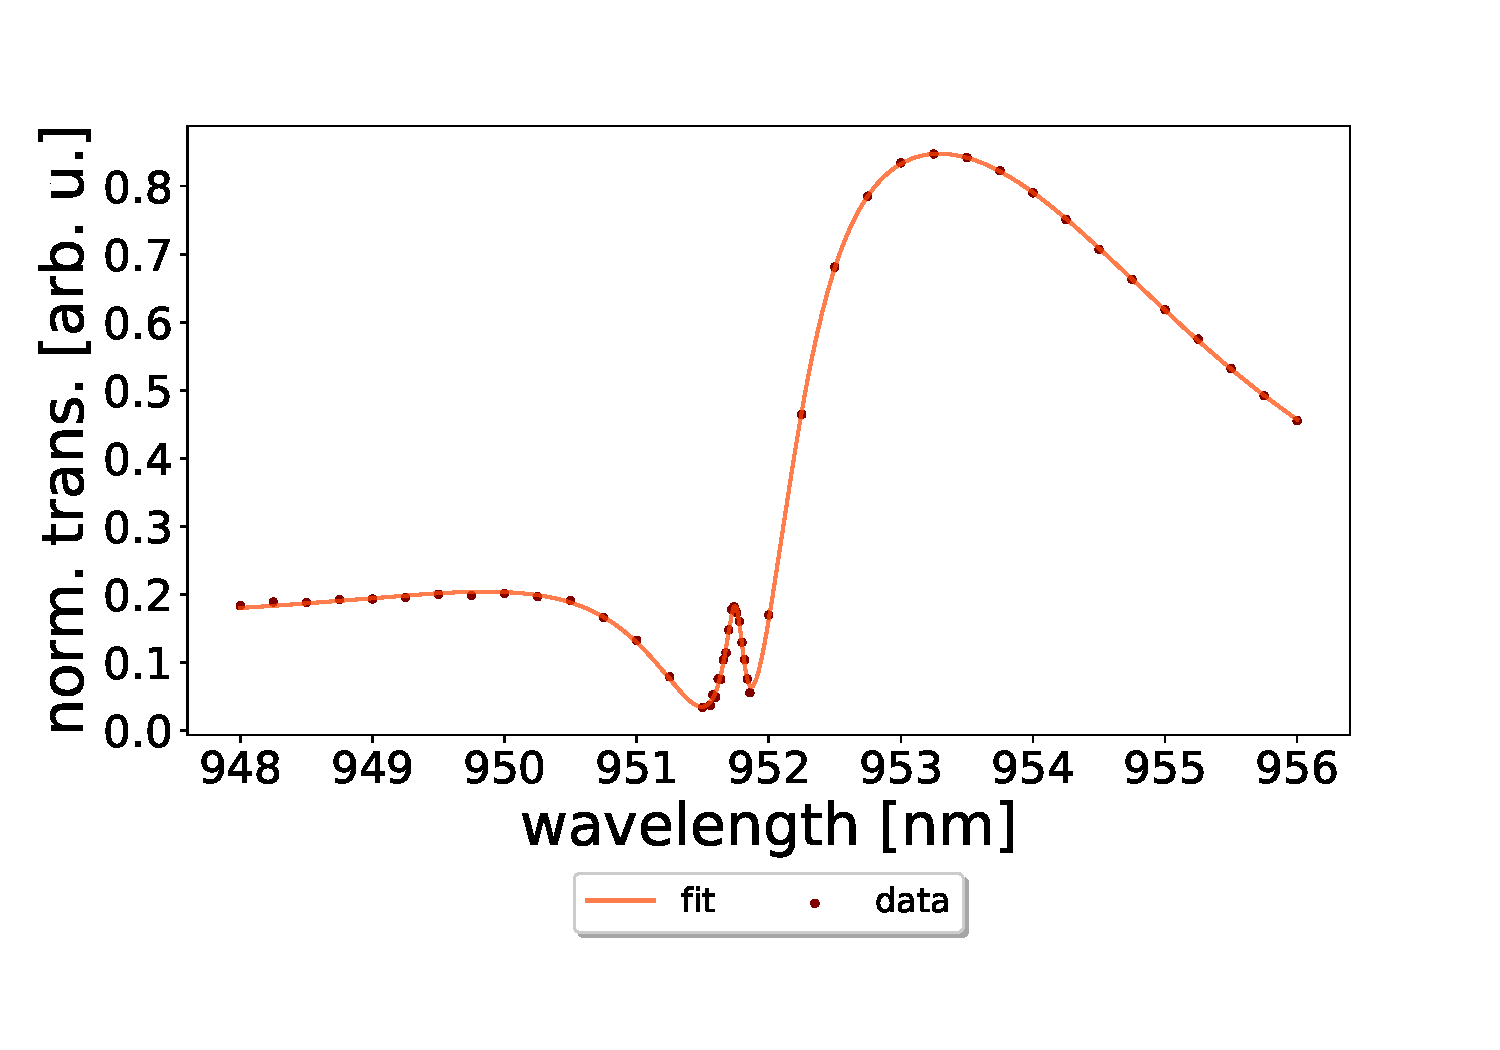
\includegraphics[width=\textwidth]{figures/results/34um_long_scan_fit.pdf}
        \caption{}
        \label{fig:34um_long_scan_fit}
    \end{subfigure}
    \caption{(a) shows recorded data of the double Fano cavity transmission compared with simulated spectra for cavity lengths of $l_{G1} = 33.3424 \mu m$, $l_{G2} = 33.3573 \mu m$ and $(l_{G1} + l_{G2})/2 = 33.3499 \mu m$. (b) shows a least squares fit of the recorded data to the double Fano cavity transmission model in eq. (\ref{eq:double_fano_transmission}).}
    \label{fig:34um_cavity_fit_and_sim}
\end{figure}

Figure \ref{fig:34um_long_scan_sim_comparison} shows the comparison of data and simulation for a cavity of lengths $l_{G1} = 33.3424 \mu m$, $l_{G2} = 33.3573 \mu m$ and $(l_{G1} + l_{G2})/2 = 33.3499 \mu m$. Figure \ref{fig:34um_long_scan_fit} shows a least squares fit of the data to the double Fano transmission function with fitting parameters related to each Fano mirror, and the cavity as follows.

Fano mirror \emph{G1} fitting parameters:
\begin{equation}
    \begin{split}
        \lambda_{0,G1} = 9&51.532 \pm 0.008 \text{nm}, \:\: \lambda_{1,G1} = 951.689 \pm 0.074 \text{nm}, \:\: t_d = 0.817 \pm 0.027, \:\: \\&\gamma_{\lambda} = 0.421 \pm 0.134 \text{nm}, \:\: \beta = 1.047 \cdot 10^{-6} \pm 4.947 \cdot 10^{-8} \text{nm}^{-1}.
    \end{split}
\end{equation}

Fano mirror \emph{G2} fitting parameters:
\begin{equation}
    \begin{split}
        \lambda_{0,G2} = 9&51.853 \pm 0.004 \text{nm}, \:\: \lambda_{1,G2} = 951.919 \pm 0.017 \text{nm}, \:\: t_d = 0.754 \pm 0.033, \:\: \\&\gamma_{\lambda} = 0.563 \pm 0.079 \text{nm}, \:\: \beta = 5.245 \cdot 10^{-7} \pm 2.823 \cdot 10^{-8} \text{nm}^{-1}.
    \end{split}
\end{equation}

Cavity parameters (length and losses):
\begin{equation}
    l = 30.984 \pm 0.006 \mu m, \:\: L = 0.017 \pm 0.184.
\end{equation}

As all parameters describing each Fano mirror and the cavity configuration are kept as variables, it is not surprising that the fit in figure \ref{fig:34um_long_scan_fit} agrees very well with the recorded data. However, even though this discredits the validity of this fit as an argument for the realization of the presented model, it is worth noting that most of the parameters agree well with the ones presented in figure \ref{fig:individual_G1_and_G2_spectra} within the estimated errors. The only exceptions are $\lambda_{0,G1}$, $\lambda_{1,G1}$ and $t_{d,G2}$, and considering that the discrepancy of the guided-mode resonance wavelength can be argued to be due to alignment variations, this fit too presents promising results for the realization of the model.

\subsubsection*{Comparison with simulations}

In all cases shown above the data and corresponding simulation mostly shows remarkable overlap and agreement, as most data points are placed within, or very close to, the area enclosed by the simulations for the three considered cavity lengths. While this is only a qualitative measure, it indicates a high level of predictive strength of the model outlined in section \ref{sec:fano_mirror} and eq. (\ref{eq:double_fano_transmission}) and likewise for the experimental method used shown in section \ref{sec:cavity_measurements}.

\subsubsection*{Fits to the double Fano model}
 
All optical parameters for G1 and G2 found as fitting parameters of the double Fano model are approximately in agreement with the ones found for G1 and G2 in section \ref{sec:results_fano_mirror_characterization} which are used to simulate the transmission spectra and assumed the baseline for determining the validity of the values found in this section. While they are only approximately in agreenment, it is noted that the values tend to shift slightly based on the alignment of the experimental setup. With this in mind the optical parameters found provide a satisfactory foundation, along with the comparisons to the simulations, to argue for the realization of the double Fano model proposed. It is my conclusion that the model performs very well in describing the recorded data. 

\subsubsection{The double fano linewidth}

As for the single Fano cavity in section \ref{sec:the_single_fano_cavity_results}, we present resonance transmission spectra and compare the found linewidths with the ones of simulated spectra and the analytical model presented in eq. (\ref{eq:analytical_linewidth_double}). The double Fano cavity realized is one comprised of Fano mirrors G1 and G2, characterized in section \ref{sec:results_fano_mirror_characterization}, in a plane-plane configuration placed normal to the optical axis. As the single Fano cavity was comprised of G1 and a HR broadband mirror, it is expected that the double Fano cavity produces spectra with broader linewidths due to the relatively higher losses. When comparing with the single Fano cavity linewidths, it must thus be noted that this is a single Fano cavity of similar losses as the double Fano cavity, and \emph{not} the one presented in section \ref{sec:the_single_fano_cavity_results}.

Figure \ref{fig:double_fano_fsr_scans} shows examples of off-resonance spectra of the double Fano cavity, with corresponding fits to the Fabry-Perot transmission function in order to determine the cavity length from the measured FSR. Figure \ref{fig:short_double_fano_FSR} shows the off-resonance spectrum for a cavity of length $l = 17.04 \pm 0.23 \mu m$, while figure \ref{fig:long_double_fano_FSR} shows the same for a cavity of length $l = 539.10 \pm 2.33 \mu m$. The errors are determined as the errors of the fits, found as the squareroot of the diagonal of the corresponding covariance matrices. 

\begin{figure}[h!]
    \centering
    \begin{subfigure}[b]{0.49\textwidth}
        \centering
        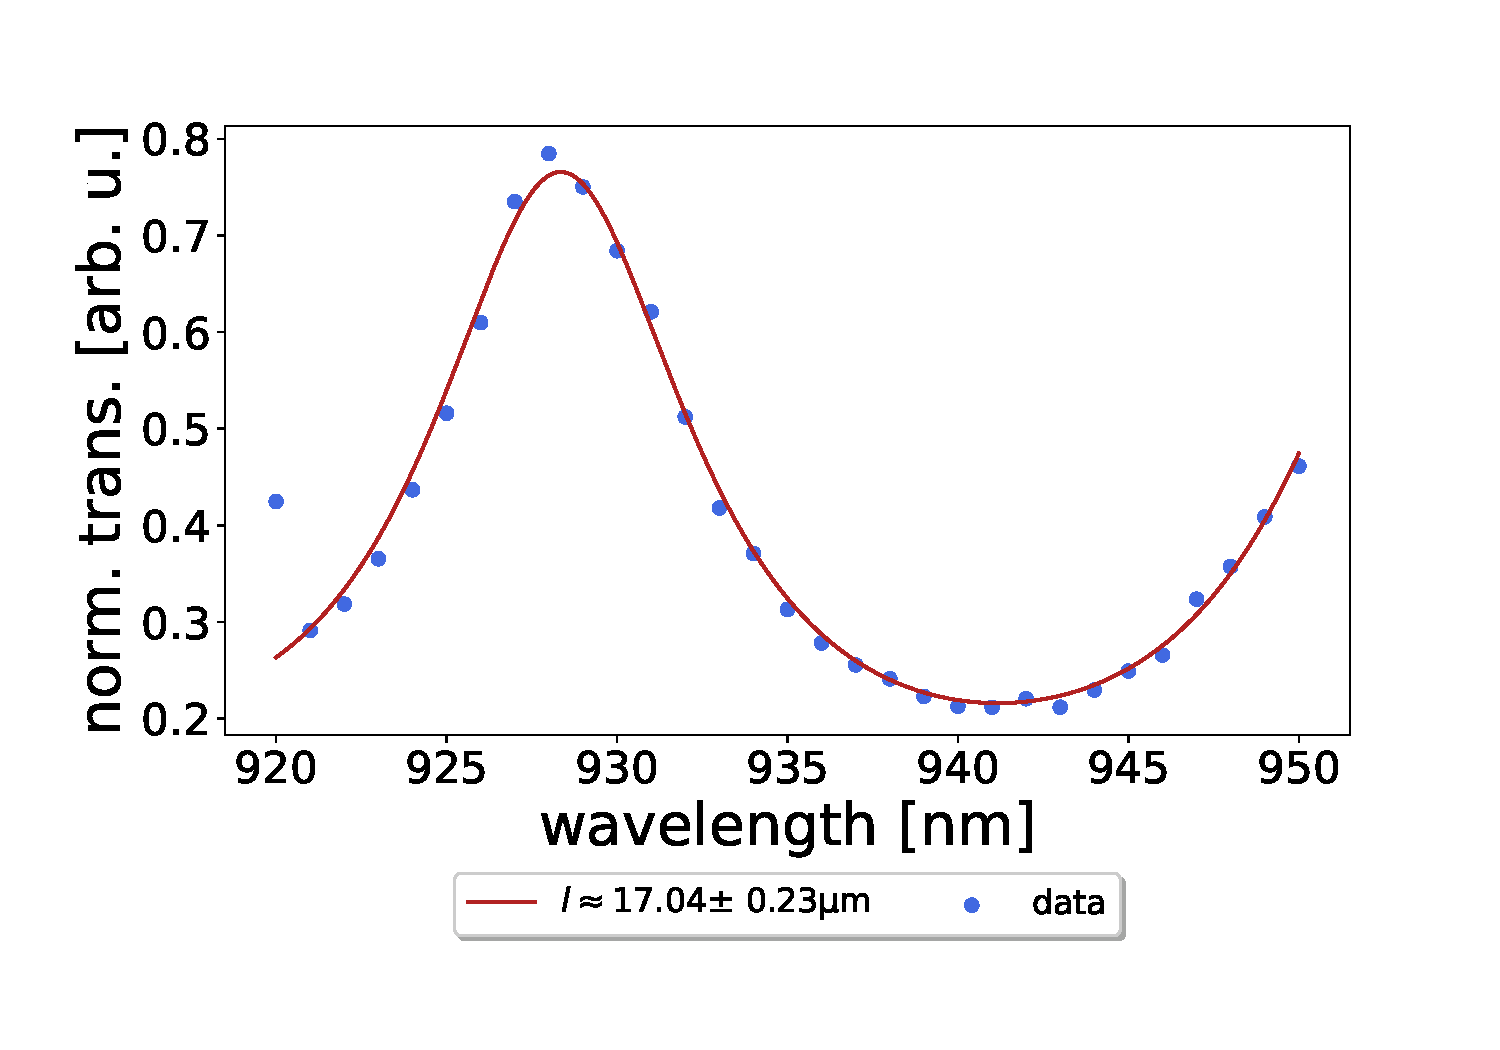
\includegraphics[width=\textwidth]{figures/results/double fano fits/30um_M3:M5_FSR_scan.pdf}
        \caption{}
        \label{fig:short_double_fano_FSR}
    \end{subfigure}
    \begin{subfigure}[b]{0.49\textwidth}
        \centering
        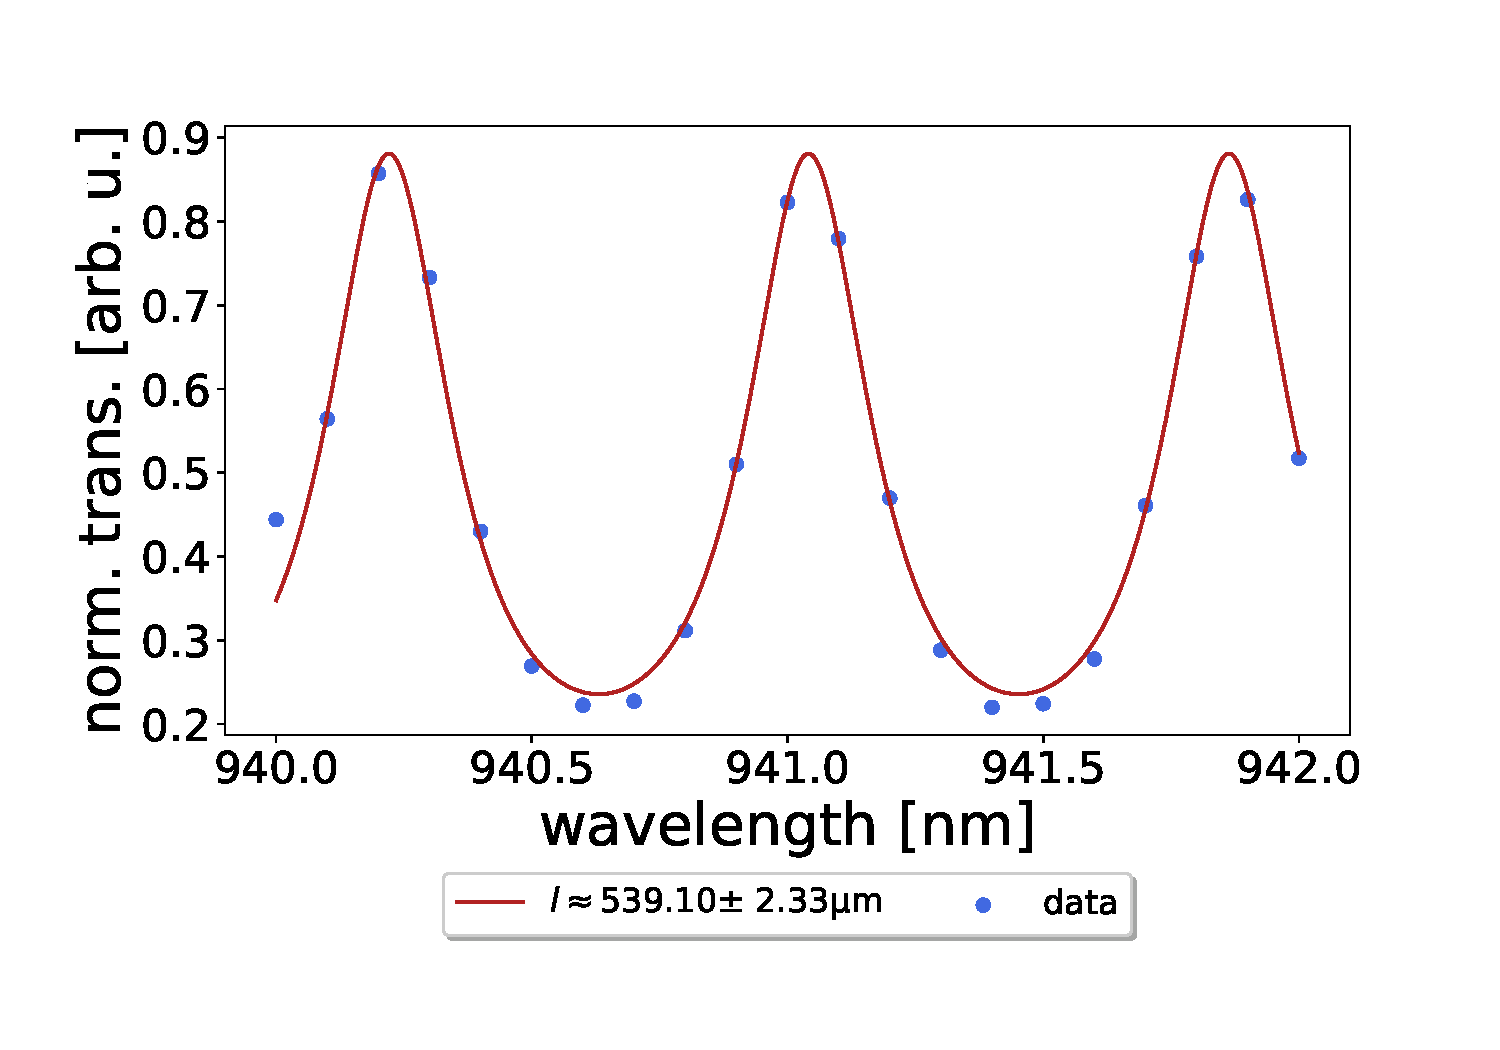
\includegraphics[width=\textwidth]{figures/results/double fano fits/550um_M3:M5_FSR_scan.pdf}
        \caption{}
        \label{fig:long_double_fano_FSR}
    \end{subfigure}
    \caption{(a) shows an off-resonance wavelength scan of the double Fano cavity consisting of a G1 and G2 for a cavity length of $l = 17.04 \pm 0.23 \mu m$. (b) shows this for a double Fano cavity of length $l = 539.10 \pm 2.33 \mu m$. Each length is determined from these measurements by measuring the FSR and utilizing that $l = \lambda_0^2/(2\cdot FSR)$.}
    \label{fig:double_fano_fsr_scans}
\end{figure}

Figure \ref{fig:double_fano_trans_data} shows examples of resonance transmission spectra of the double Fano cavity. The examples are taken for length corresponding to the ones found from the off-resonance spectra shown in figure \ref{fig:double_fano_fsr_scans} above. The figures are depicted with each their corresponding least squares fits to the generalized Fano model shown in eq. (\ref{eq:general_fano_model}) in order to determine the linewidth (HWHM) of the profile. The errors of the linewidths are found from the error of each fit and are mainly used to determine the quality of the measurement. 

\begin{figure}[h!]
    \centering
    \begin{subfigure}[b]{0.49\textwidth}
        \centering
        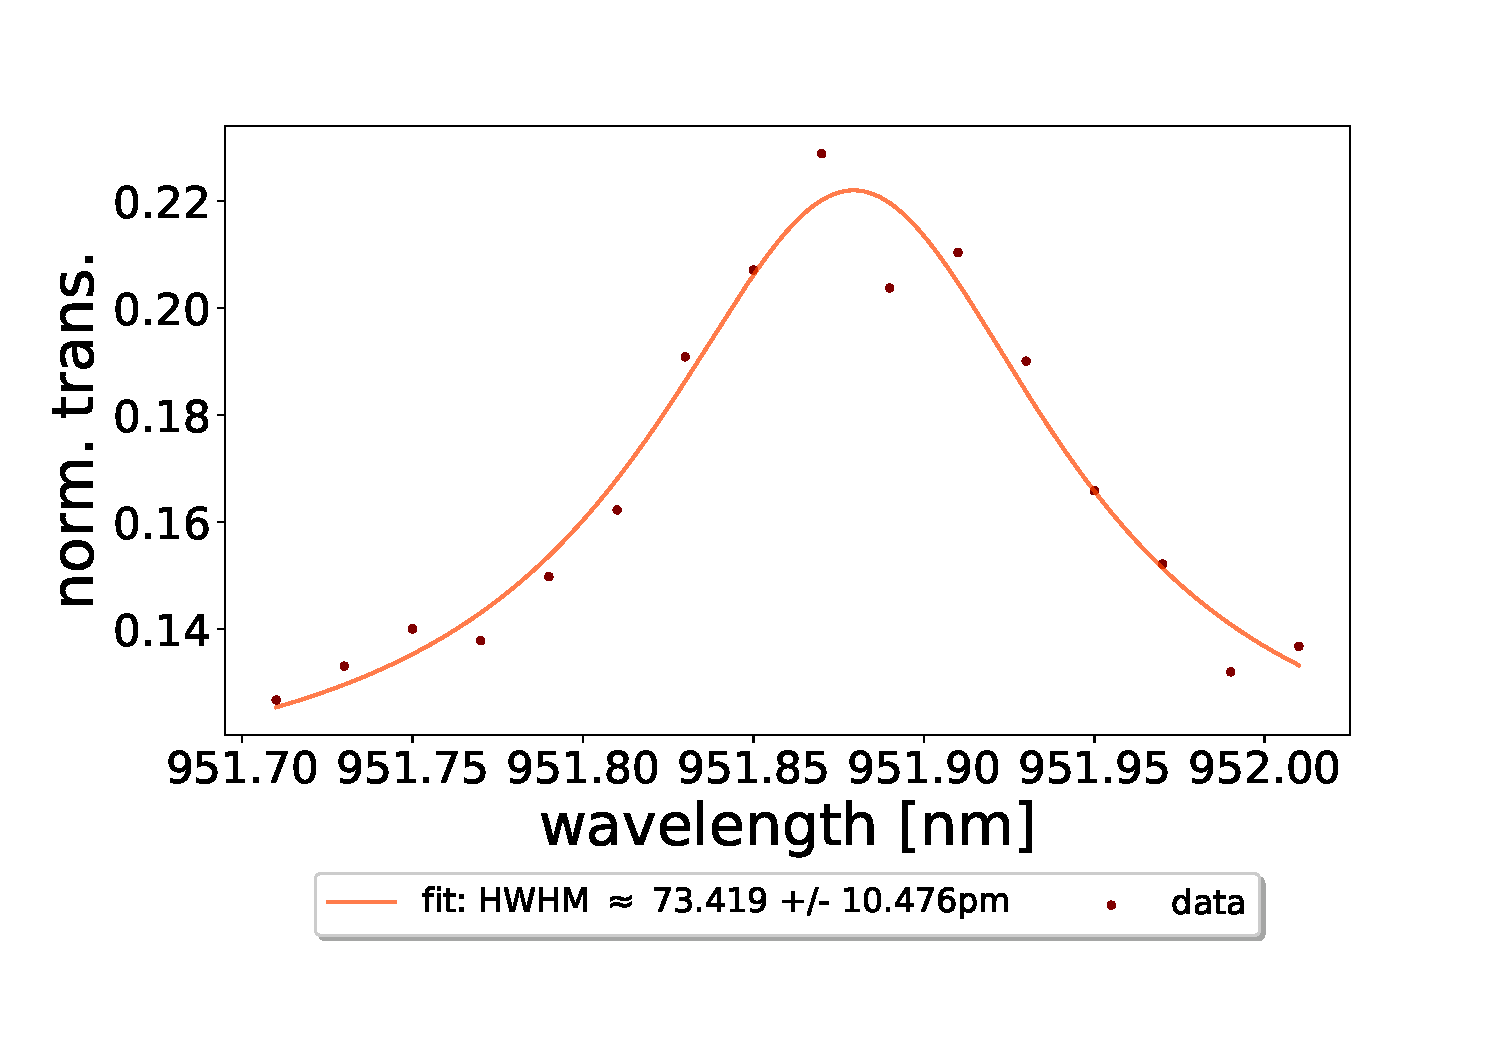
\includegraphics[width=\textwidth]{figures/results/double fano fits/30um_M3:M5_fit_4.pdf}
        \caption{}
        \label{fig:short_double_fano_trans}
    \end{subfigure}
    \begin{subfigure}[b]{0.49\textwidth}
        \centering
        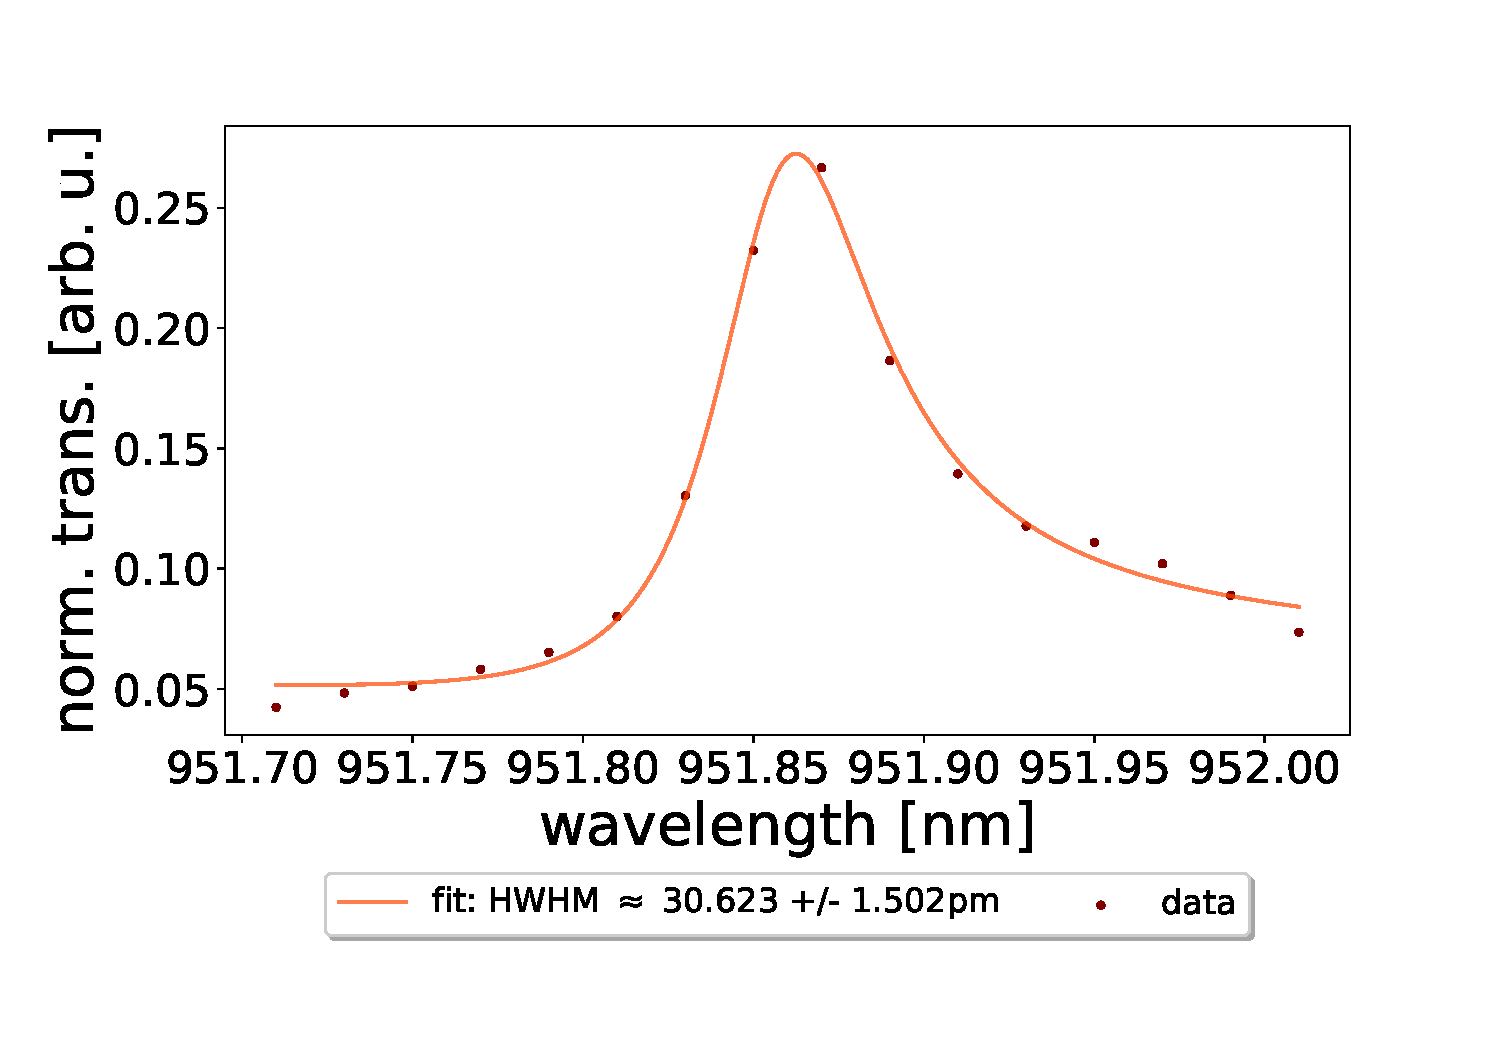
\includegraphics[width=\textwidth]{figures/results/double fano fits/550um_M3:M5_fit_1.pdf}
        \caption{}
        \label{fig:long_double_fano_trans}
    \end{subfigure}
    \caption{Double Fano resonance transmission profiles of a cavity consisting of Fano mirrors G1 and G2. (a) shows the profile of a cavity of length $l = 17.04 \pm 0.23 \mu m$ and displays a linewidth of $HWHM = 73.419 \pm 10.476$pm. (b) shows the profile of a cavity of length $l = 539.10 \pm 2.33 \mu m$, with a linewidth of $HWHM = 30.623 \pm 1.502$pm.}
    \label{fig:double_fano_trans_data}
\end{figure}

Figure \ref{fig:HWHM_vs_l_double_fano_result} shows the average of results for the linewidths of a number of recorded spectra taken for cavity lengths in the approximate range $15 \mu m \leq l \leq 1000 \mu m$. The error of each data point depicted is determined as the standard deviation of all values found for the linewidth at that particular cavity length. The error in the x-direction, i.e. for the cavity lengths found from fits as the ones shown in figure \ref{fig:double_fano_fsr_scans} were of negligible size and are thus indicated rightly in the size of the data points themselves. The blue dashed line depicts the analytical linewidth of a broadband cavity of losses similar to the double Fano cavity realized experimentally, the line is calculated using eq. (\ref{eq:analytical_linewidth_broadband}). The orange dashed line similarly shows the analytical linewidth of the single Fano cavity calculated using eq. (\ref{eq:analytical_linewidth_single_fano}) for a cavity of similar losses. Lastly, the green dashed line indicates the analytical linewidth of the double Fano cavity transmission spectra comparable with the data points depicted. The black points are linewidths found by fitting double Fano transmission profiles simulated using eq. (\ref{eq:double_fano_transmission}) to the generalized Fano model in eq. (\ref{eq:general_fano_model}) for comparison.

\begin{figure}[h!]
    \centering
    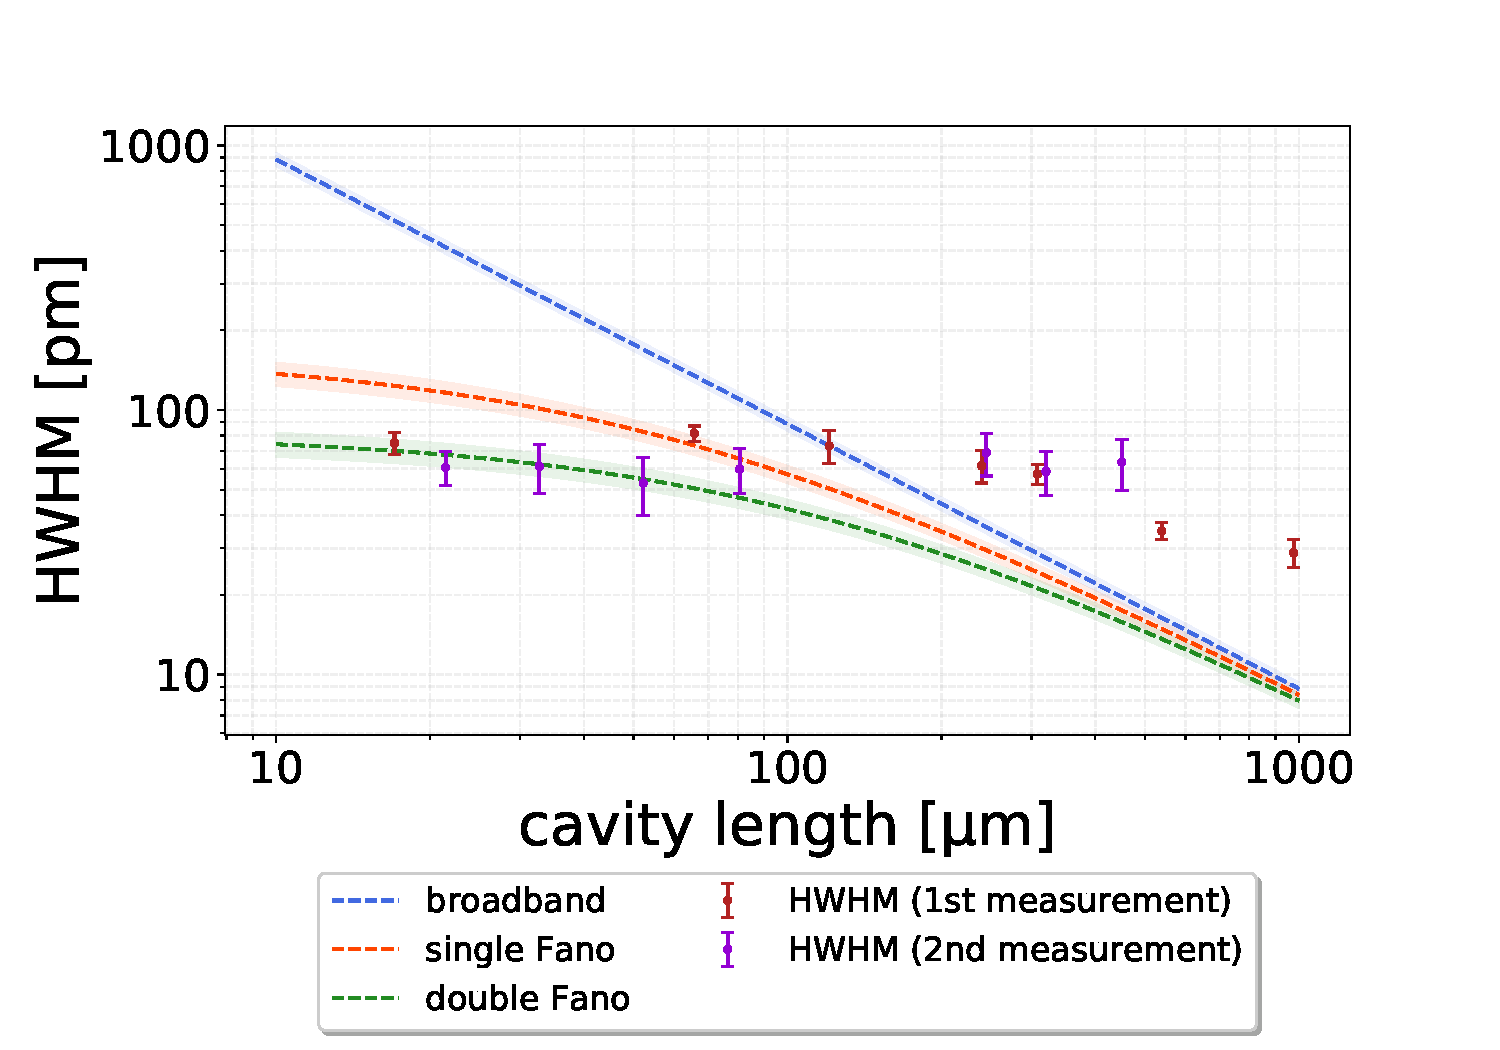
\includegraphics[width=0.7\textwidth]{figures/results/double fano fits/HWHM_vs_cavity_length_result.pdf}
    \caption{The linewidth (HWHM) as a function of resonant cavity length. The blue, orange and green dashed lines show the analytical linewidths of a broadband, single Fano and double Fano cavity of similar losses calculated using eqs. (\ref{eq:analytical_linewidth_broadband}), (\ref{eq:analytical_linewidth_single_fano}) and (\ref{eq:analytical_linewidth_double}). The optical parameters for G1 and G2 used for these calculations are determined from spectra rerecorded on the same day as the linewidth measurements for optimal comparison, this will be discussed in section \ref{sec:additional_discussion}. The dark red point and corresponding errorbars shows the measured linewidths found as averages of all recorded values at each length and the error is found as the standard deviation of these. The black points are the linewidths of simulated spectra. The spectra used to determine the points depicted can be found in Appendix \ref{appendix:Measured double Fano transmission data}.}
    \label{fig:HWHM_vs_l_double_fano_result}
\end{figure}

It is seen that the analytical and simulated linewidths are strongly correlated, which indicates that both describe the transmission spectra well. This is also indicated in section \ref{sec:realizing_the_double_fano_model} where the realization of the double Fano model is shown to correlate well with the spectra produced. However, when examining the measured linewidths of the double Fano cavity resonance transmission profile, it is clear that it deviates from the analytical and simulated ones. The double Fano cavity has shown to be very sensitive to vibrational and acoustic noise, and this becomes more apparent when increasing the cavity length. Note that the correlation between the analytical and measured linewidths becomes correspondingly stronger for decreasing cavity lengths, and that they overlap almost completely when considering the spectra at $l \approx 17 \mu m$. This indicates that analytical double Fano cavity linewidths are roughly realizable inside the Fano regime. It is also noted that the behavior of the measured linewidth as a function of cavity length follows the trend of the analytical one, indicating that the Fano and standard regimes are still applicable for the double Fano cavity. 

While vibrational and acoustic noise definitely claims their part of the reason for the experienced broadening, the method used to align the double Fano cavity outlined in section \ref{sec:alignment} too has potential for improvement. When going through the process of aligning the cavity, one relies on the assumption that the top and bottom parts of the cavity setup can be removed and reinserted without loss of alignment in either of the numerous degrees of freedom. This is of course not always the case and is therefore a cause of misalignment of the cavity and thus broadening. 

Designing a setup and method with complete independent control of all degrees of freedom is therefore an area of improvement that could likely reduce the dicrepancy of the analytical/simulated and measured linewidths of the double Fano cavity resonance transmission spectra.

\subsection{Additional discussion}\label{sec:additional_discussion}

\subsubsection{Vibrational noise}

The aforementioned vibrational noise was apparent from the intial iteration of the double Fano cavity setup and it was quickly concluded that it was specifically related to the modifications made to the single Fano cavity setup in order to be able to control additional degrees of freedom needed. 

\begin{figure}[h!]
    \centering
    \begin{subfigure}[b]{0.49\textwidth}
        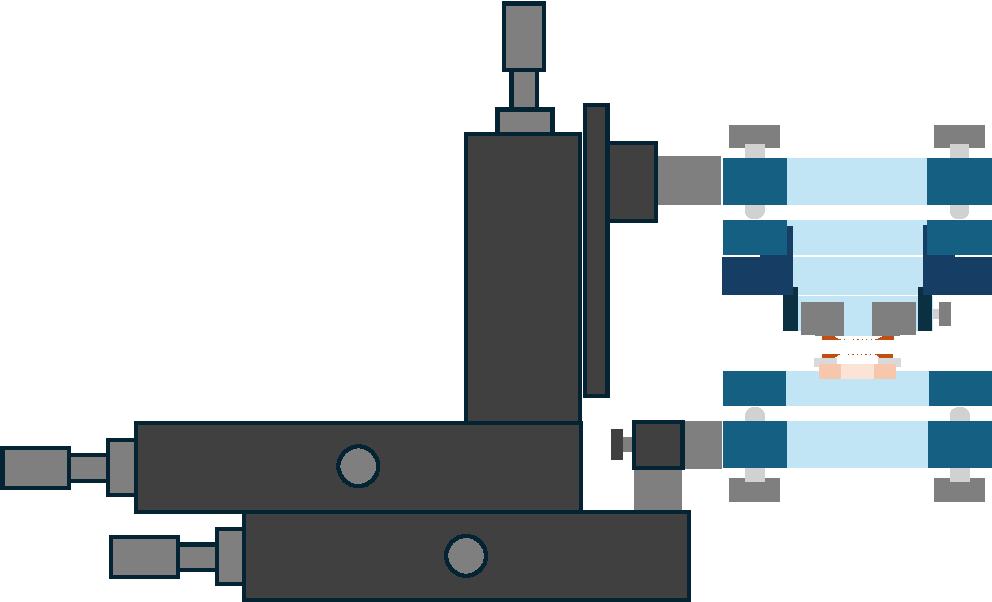
\includegraphics[width=\textwidth]{figures/double_fano_sketch_discussion.pdf}
        \caption{}
        \label{fig:double_fano_discussion}
    \end{subfigure}
    \begin{subfigure}[b]{0.49\textwidth}
        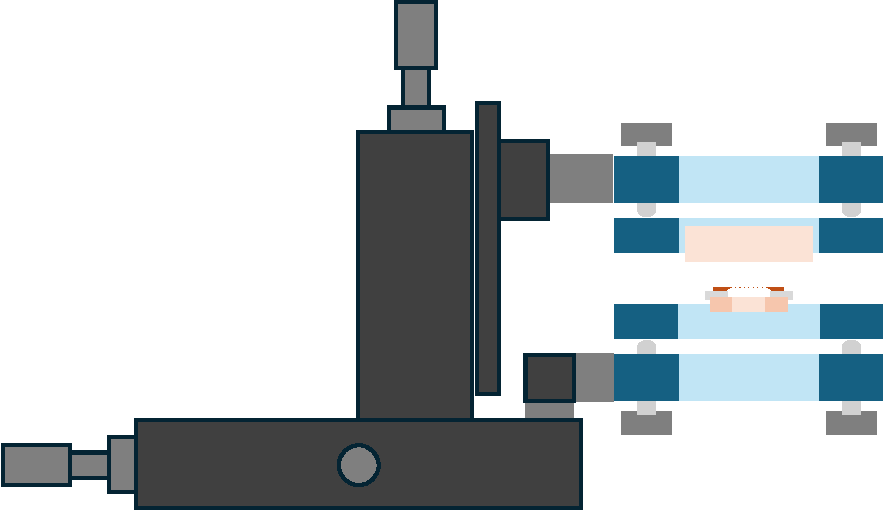
\includegraphics[width=\textwidth]{figures/single_fano_sketch_discussion.pdf}
        \caption{}
        \label{fig:single_fano_discussion}
    \end{subfigure}
    \caption{Simple sketches of the setups used to record the data shown in sections \ref{sec:the_single_fano_cavity_results} and \ref{sec:the_double_fano_cavity_results}. (a) shows the double Fano cavity setup, and (b) shows the single Fano cavity setup.}
    \label{fig:single_vs_double_sketch}
\end{figure}

Especially the translational degrees of freedom seemed to be the source of the vibrations, as the need to control these for the bottom and top Fano mirrors independently introduced the possibility of \emph{uncoupled mechanical vibrations}. It is assumed that the noise was always apparent in the setup, but since the broadband and Fano mirrors of the single Fano cavity only ever had the need for relative motion in the z-direction, this was never expressed as a change in the cavity length, and this was thus constant during measurements. The linear stage used in the z-direction (\emph{NFL5DP20}) was specifically chosen to include a piezo actuator for high resolution motion control for very short cavity lengths, and this proved to be virtually stable in terms of vibrations. While a number of different stages, with a longer maximum travel range, was tested for the xy-directions, none proved stable enough to completely cancel the uncoupled vibrations. Figure \ref{fig:single_vs_double_sketch} shows sketches of the single and double Fano cavity setups and it is here shown how the top and bottom of the setup was \emph{uncoupled} through the addition of the xy-stages for aligning the top Fano mirror, while for the single Fano setup they were \emph{coupled} as they were both attached to the same set of xy-stages. 

\begin{figure}[h!]
    \centering
    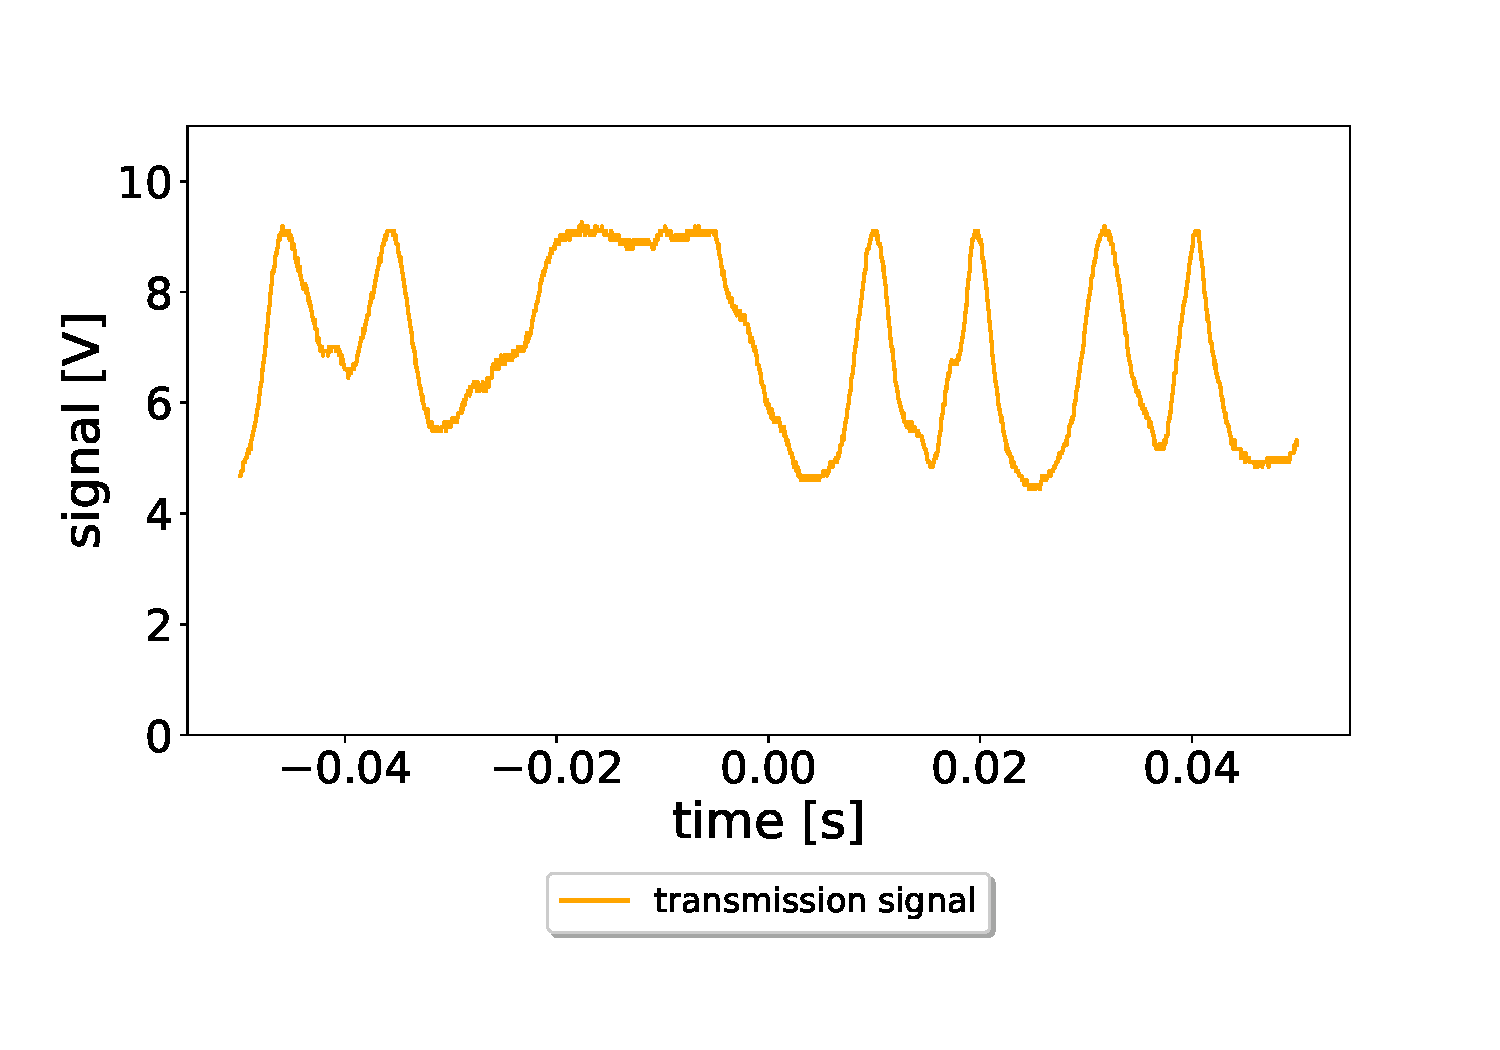
\includegraphics[width=0.7\textwidth]{figures/results/noise_on_resonance.pdf}
    \caption{ An example of the signal measured of the double Fano cavity transmission when manually scanning the piezo actuator to tune the cavity and guided-mode resonances. It is assumed that the cavity is resonant when the signal is maximized and thath the fluctuations is due to vibrational noise. This naturally causes broadening and its effect is therefore apparent in the results presented.}
    \label{fig:noise_on_resonance}
\end{figure}

Initially, the vibrations had an amplitude comparable with the free stroke of the piezo actuator. This means that the fringes stemming from scanning the cavity length would hardly change when turning off the alternating current applied to the actuator, and thus a stable measurement was deemed impossible. At this point it was unclear whether the noise was acoustic in nature or if the vibrations originated somehow from the optical table. To rule out, or reduce, acoustic vibrations the setup was enclosed inside a plexi-glas box which was further equipped with a piece of noise reducing foam. This addition proved helpful as it roughly reduced the amplitude of the noise by a factor of $2$, thus making the spectral profile resolvable and measurements possible. 

Additional measures were taken to reduce any vibrations originating from the optical table by the addition of teflon slabs between the optical table and the first set of xy-stages, and between these and the second set of xy-stages. This further reduced the noise slightly and the resulting signal, shown as the raw data from the oscilloscope screen, is seen in figure \ref{fig:noise_on_resonance}.

It is assumed that the optimal cavity length is the one that produces the highest signal when the cavity length is constant. Keeping this in mind it is easily deduced from the figure that further noise reduction will increase the quality of the meaured spectra. Since the intrinsicly narrower linewidths produced by longer optical cavities (both standard and Fano) makes these more sensitive to noise as the kind depicted in figure \ref{fig:noise_on_resonance}, this hints towards an explanation for the increased deviation from the analytical linewidth for longer cavity lengths seen in figure \ref{fig:HWHM_vs_l_double_fano_result}.

A brief decsription of the plexiglas box and teflon slabs are found in section \ref{sec:vibrational_noise_reduction}.

\begin{figure}[h!]
    \centering
    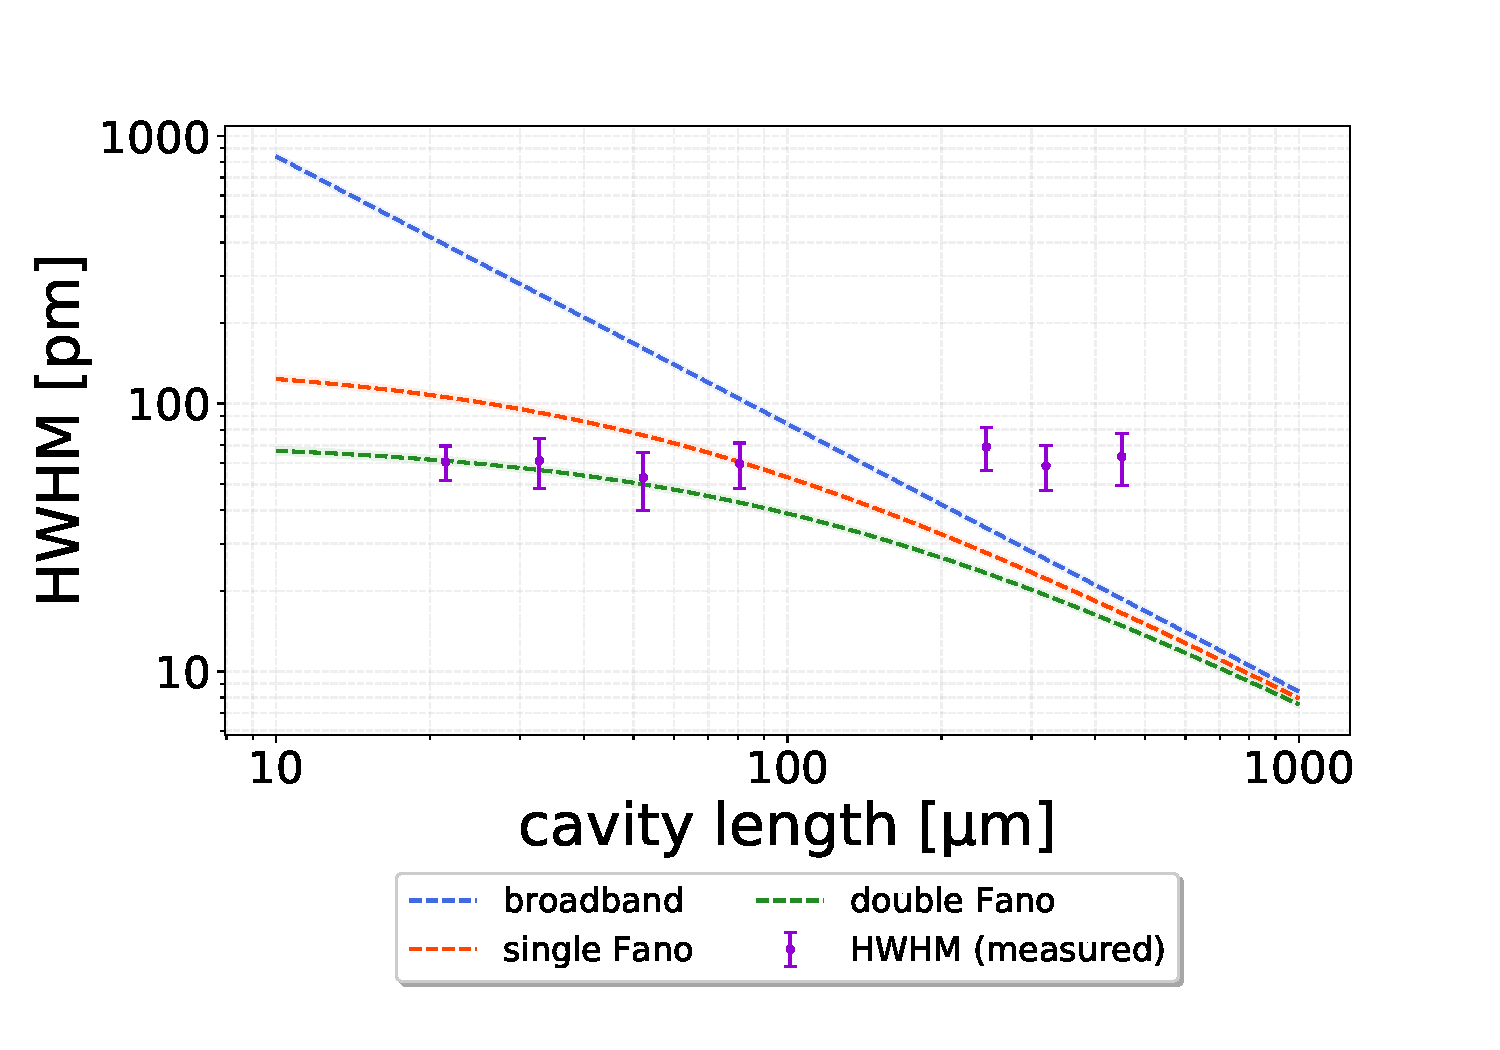
\includegraphics[width=0.7\textwidth]{figures/results/double fano fits/HWHM_vs_cavity_length_result_2nd_measurement_only.pdf}
    \caption{A measurement series showing the best obtained results for the double Fano cavity transmission linewidth as a functio of resonant cavity length. This measurement series was recorded \emph(before) the addition of the teflon slabs, which where added in an attempt to create a reflective interface to shield the cavity from vibrations propergating throught the optical table. The spectra used to determine the points depicted can be found in Appendix \ref{appendix:Measured double Fano transmission data}.}
    \label{fig:HWHM_vs_l_double_fano_noisy}
\end{figure}

Figure \ref{fig:HWHM_vs_l_double_fano_noisy} shows the best obtained measurement series taken with the setup \emph{without} teflon slabs, and while the cavity lengths considered does not range as far as the measurement series in figure \ref{fig:HWHM_vs_l_double_fano_result}, the trend of increased broadening in the standard regime is apparent. It also shows that even for the case of increased vibrational noise, it is possible to record spectra of linewidths in agreement with the analytical prediction, when inside the Fano regime. Note here that the errorbars on the figure are representative of the standard deviations of all values recorded at each cavity length, and thus the noisy measurement is seen to fluctuate more resulting in higher uncertainties. 

\newpage
\subsubsection{Guided-mode resonance shift}

\begin{figure}[h!]
    \centering
    \begin{subfigure}[b]{0.49\textwidth}
        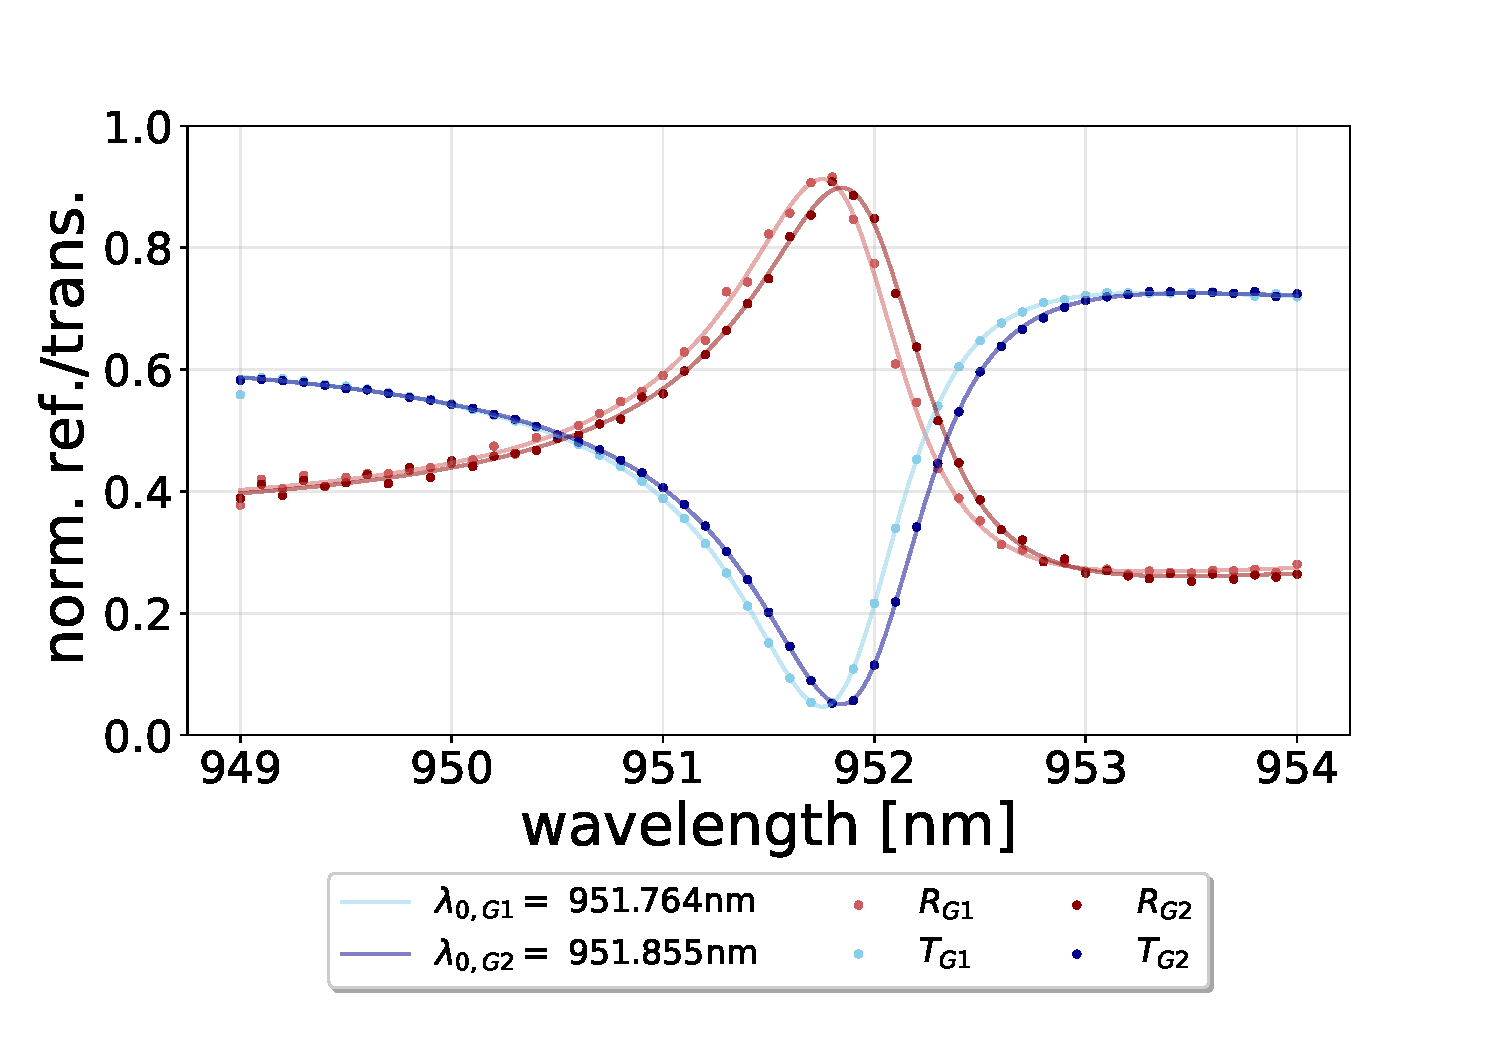
\includegraphics[width=\textwidth]{figures/results/M3:M5/M3:M5_initial_spectra.pdf}
        \caption{}
        \label{fig:G1_and_G2_initial_discussion}
    \end{subfigure}
    \begin{subfigure}[b]{0.49\textwidth}
        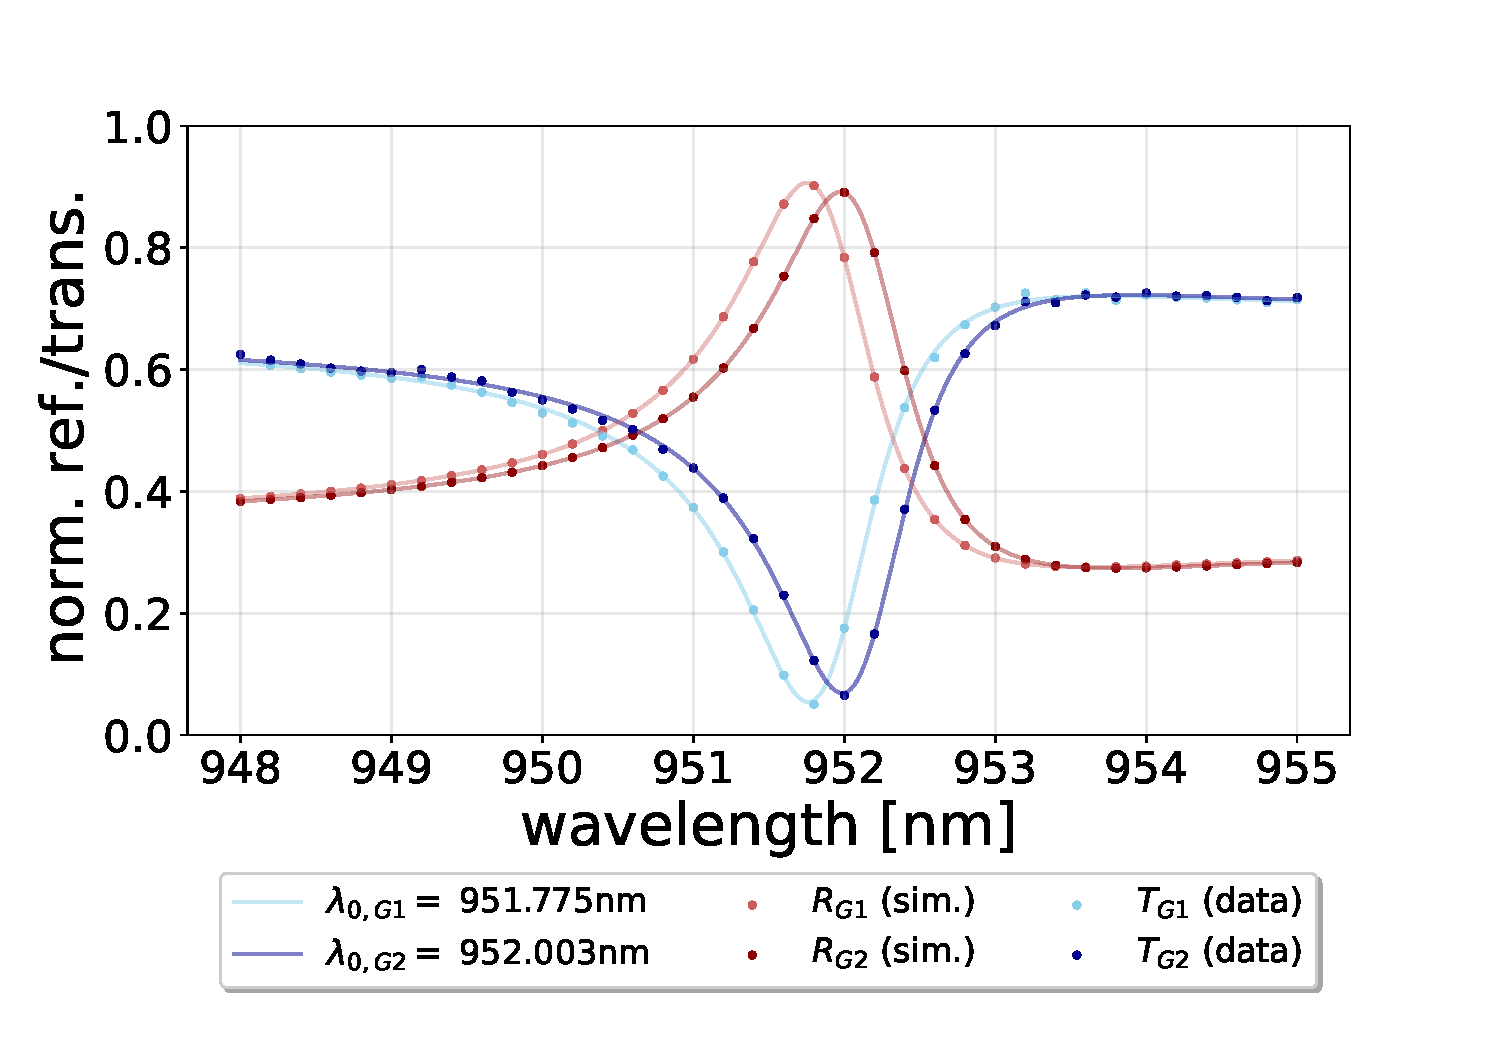
\includegraphics[width=\textwidth]{figures/results/M3:M5/M3:M5_spectra_at_measurement.pdf}
        \caption{}
        \label{fig:G1_and_G2_double_fano_config_discussion}
    \end{subfigure}
    \caption{(a) shows spectra of G1 and G2 measured individually. (b) shows spectra of G1 and G2 in the double Fano configuration at a later time.}
    \label{fig:G1_and_G2_spectra_individual_and_in_double_fano_config}
\end{figure}

The spectra for G1 and G2 shown in figure \ref{fig:G1_and_G2_spectral_comparison} are taken individually and in the intial part of the project where finding a matching pair of Fano mirrors was the task at hand. Figure \ref{fig:G1_and_G2_initial_discussion} shows, once again, the spectra of G1 and G2 taken individually, while figure \ref{fig:G1_and_G2_double_fano_config_discussion} shows spectra taken for the two in the double Fano configuration at a later time.

It is apparent that while the spectra for G1 is virtually unchanged, the same cannot be said for the spectra of G2 as this has clearly shifted to a slightly higher guided-mode resonance. This artifact has been observed several times in both this project and related projects in the same lab, as the resonance wavelength of \emph{some} SiN sub-wavelength gratings tends to shift with time. An in depth investigation of this behavior have to my knowledge not been conducted, however it is something that must be taken into account when evaluating recorded data. One considerable consequence of this is that all data presented must be recorded in the same measurement series, as measurements done on different days cannot be compared. It must be noted that the resonant guided-mode wavelength is very dependent on the alignment of a given Fano mirror, which could influence this behavior, it is however also apparent that the resonance tends to systematically shift to higher wavelengths only. 

For optimal comparison, the parameters used to calculate the analytical linewidths in figures \ref{fig:HWHM_vs_l_double_fano_result} and \ref{fig:HWHM_vs_l_double_fano_noisy} are found as fitting parameters of spectra recorded on the same day as the measurements included in the each figure. The analytical linewidths have shown to only differ slightly for different spectra for G1 and G2, but the discrepancy is nontheless not negligible and must hence be considered.

\subsubsection{Potential broadening due to walk-off effect}

Another potential source of broadening is the so-called \emph{walk-off effect} which is apparent, in this case, for the scenario of a wedge angle between G1 and G2. For a non-zero wedge angle the beam will be reflected inside the cavity and propagate according to said wedge angle as simply sketched in figure \ref{fig:walk_off_sketch}. This would result in an effective change in the translational alignement of the beam relative to the Fano mirror/cavity, and thus broadening of the recorded spectra.

\begin{figure}[h!]
    \centering
    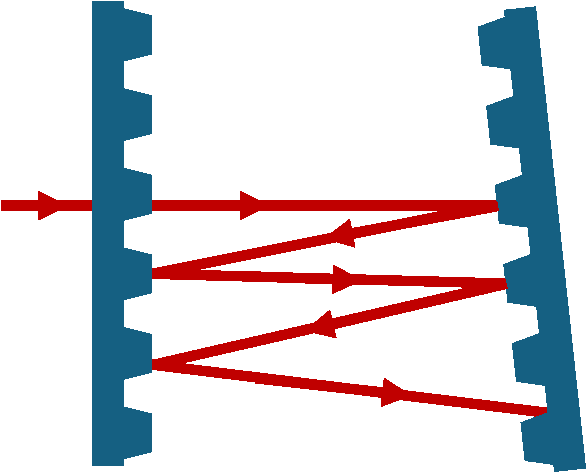
\includegraphics[width=0.4\textwidth]{figures/walk_off_sketch.pdf}
    \caption{Sketch illustrating the walk-off effect between two Fano mirrors at a non-zero wedge angle.}
    \label{fig:walk_off_sketch}
\end{figure}

A small, if not negligible, wedge angle is assumed for any experimentally realized cavity, but for the double Fano cavity with a non-zero detuning $\Delta$ this might be enhanced by the method it self. In \cite{Parthenopoulos} it is shown that the resonance wavelength will increase for a Fano mirror of a non-zero incident angle at the cost of a higher (lower) minimum (maximum) transmission (reflectivity) when on resonance. The argument can be made that the optimal double Fano configuration for a non-zero detuning is not necessarily normal to the optical axis, but rather at a wedge angle which optimizes the spectral overlap of the two Fano mirrors. For this reason the angle between G1 and G2 might be increased when on-resonance measurements are recorded and hence the walk-off effect might contribute to the broadening seen in figure \ref{fig:HWHM_vs_l_double_fano_result}. The walk-off effect will, if apparent, naturally increase with the cavity length, as a simple geometric consequence of the configuration considered. 
